% !TEX root = ../../main.tex
\chapter{Results}
\label{ch:results}

The results after performing the statistical analysis outlined in \Ch{\ref{ch:stats}} are presented in this chapter. In~\Sect{\ref{sec:results:bkgonly}}, a background-only fit is performed to the data. Signal region $m(\ell\nu J)$ distributions, event yields for observed data and all fitted SM backgrounds, and the fitted normalizations for the \Wjets and \ttbar backgrounds are presented. In~\Sect{\ref{sec:limits}}, model-dependent fits are performed using the profile likelihood ratio to set upper limits on the expected and observed cross sections times branching ratio to $WV$, for the selected benchmark signal models. The systematic uncertainties (\Ch{\ref{ch:syst}}) with the largest impact on the signal strength fits are discussed. Event displays showcasing signal region events with the highest invariant mass are presented in \App{\ref{ch:eventDisplay}}.


%%
\section{Background-Only Fit} 
\label{sec:results:bkgonly}
No significant excesses above the SM prediction are observed after the simultaneous binned likelihood fit to the data with the background-only hypothesis (fixed signal strength $\mu=0$). The post-fit $m(\ell\nu J)$ distributions for the VBF selection are shown for the HP and LP regions in~\Fig{\ref{fig:pf_hp_vbf}} and~\Fig{\ref{fig:pf_lp_vbf}}, respectively. The corresponding distributions for the ggF selection are shown for the HP and LP regions in~\Fig{\ref{fig:pf_hp_ggf}} and~\Fig{\ref{fig:pf_lp_ggf}}, respectively. Pre-fit signal distributions for $m=2\,\TeV$\, ($m=1.2\,\TeV$) are overlaid for the ggF (VBF) selection regions. The total post-fit uncertainty, accounting for both statistical uncertainties and systematic uncertainties, is included. 

% Post fit plots
\begin{figure}[htb]
\centering
\subfloat[]{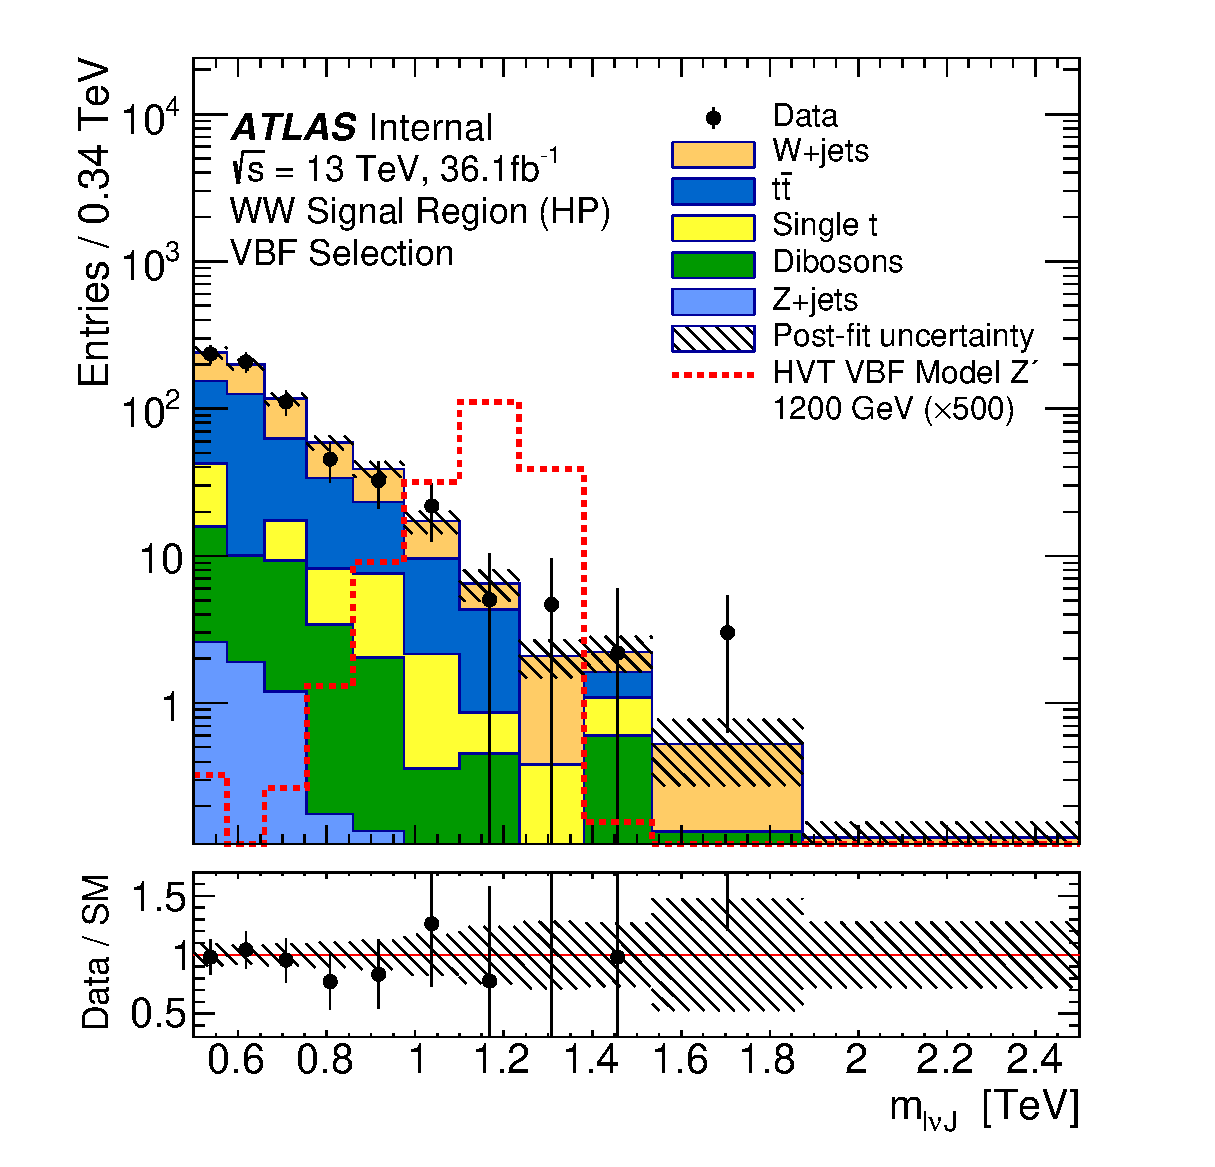
\includegraphics[width=.48\textwidth]{figures/Results/new/final_pf/postFit_VBF_HVTWW_1000_SRWW_HP}\label{fig:pf_hp_vbf:a}}
\subfloat[]{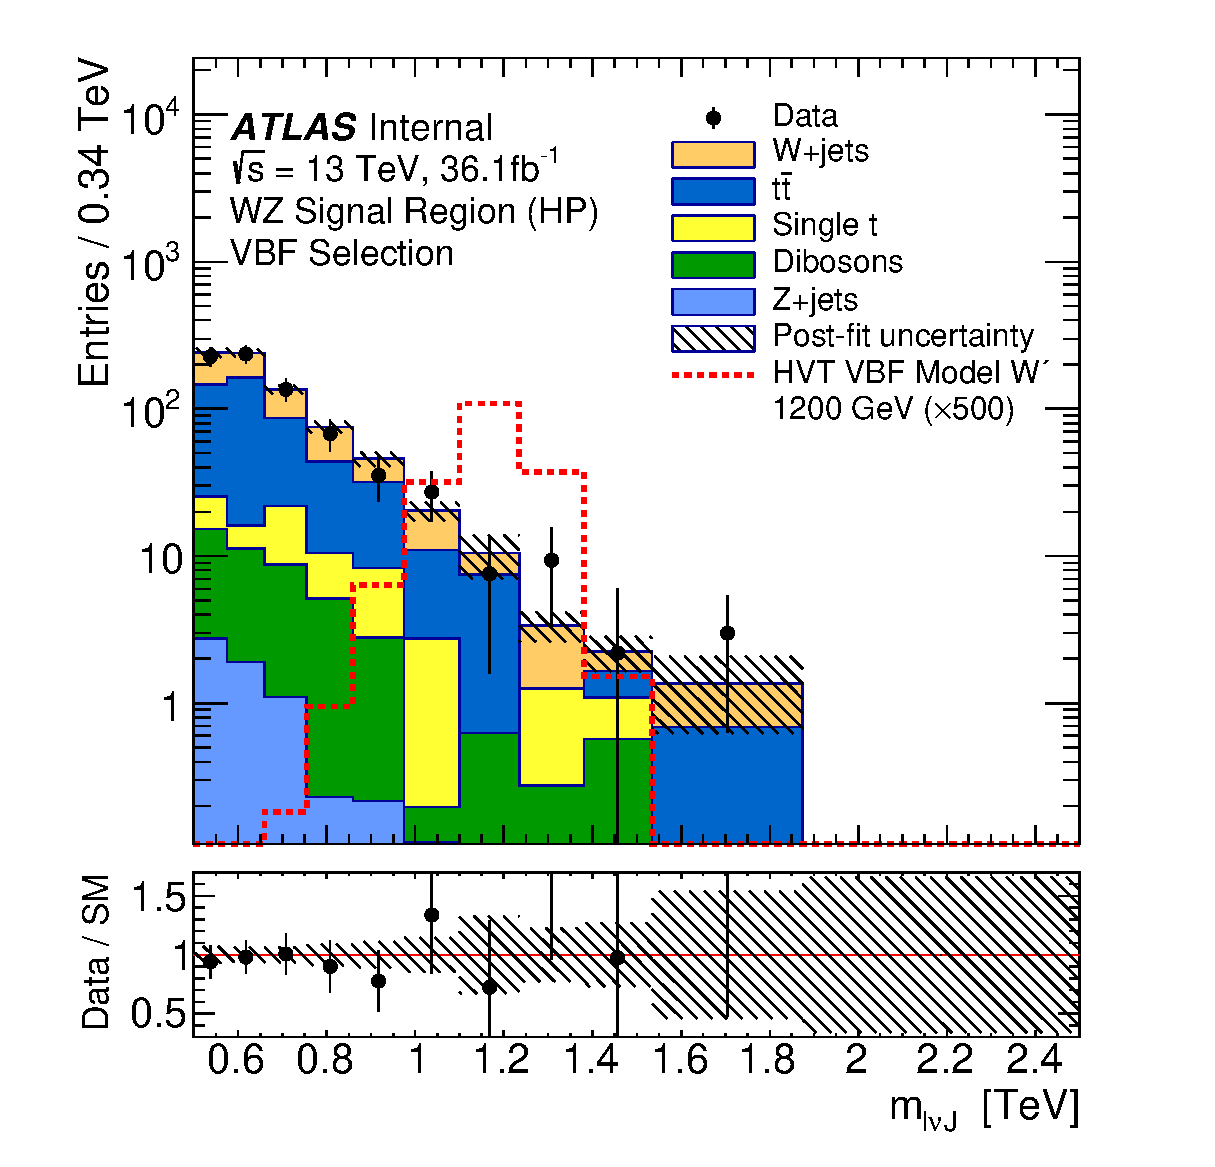
\includegraphics[width=.48\textwidth]{figures/Results/new/final_pf/postFit_VBF_HVTWZ_1000_SRWZ_HP}\label{fig:pf_hp_vbf:b}}\\
\subfloat[]{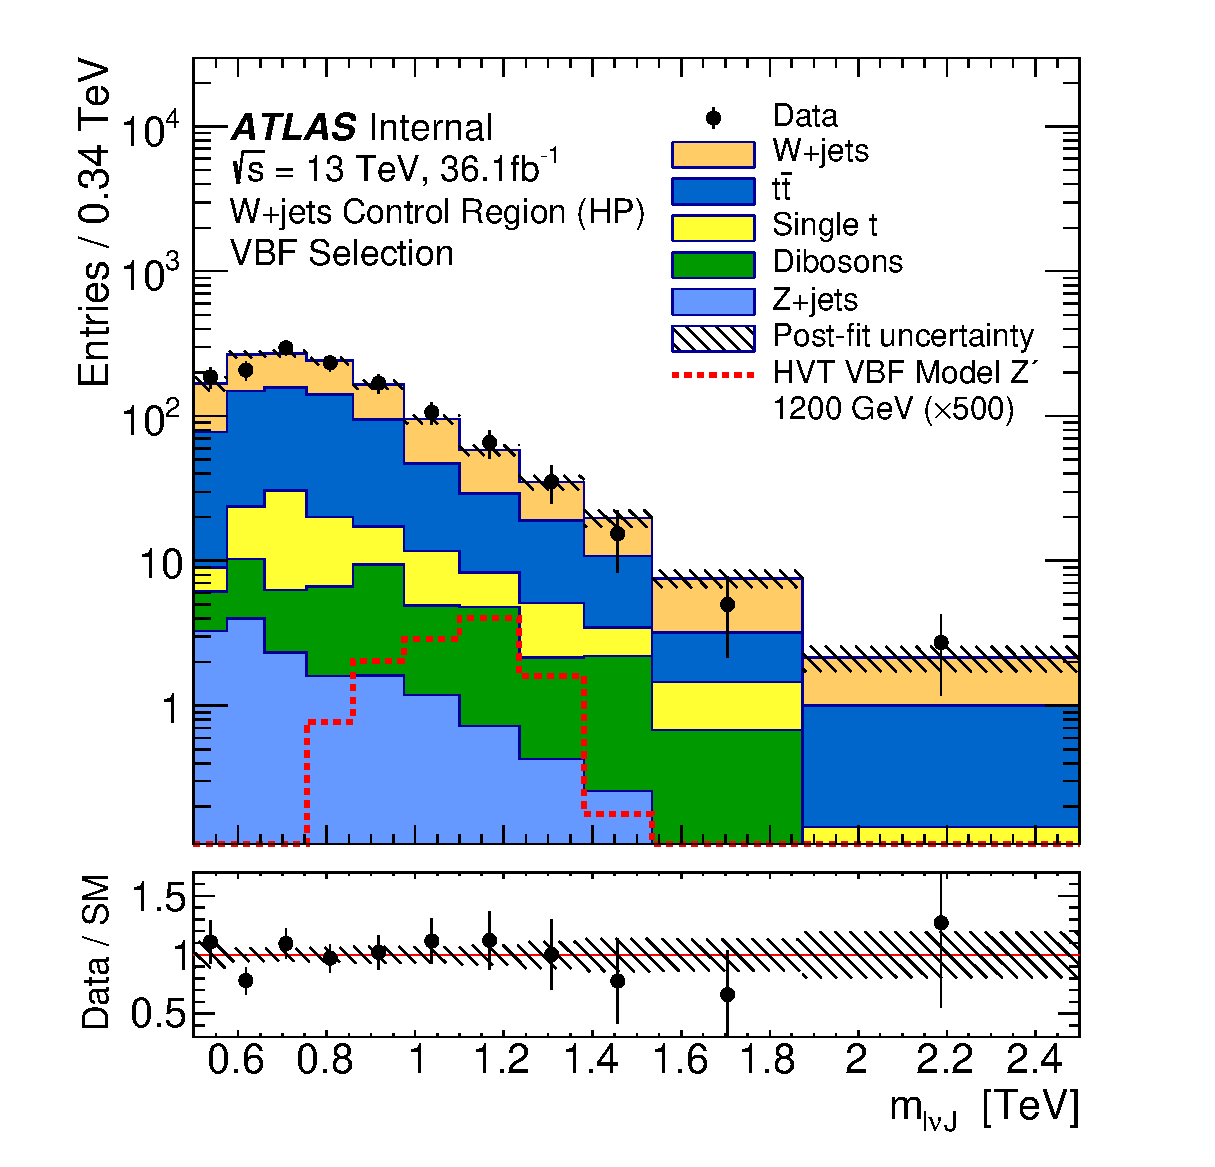
\includegraphics[width=.48\textwidth]{figures/Results/new/final_pf/postFit_VBF_HVTWW_1000_WCR_HP}\label{fig:pf_hp_vbf:c}}
\subfloat[]{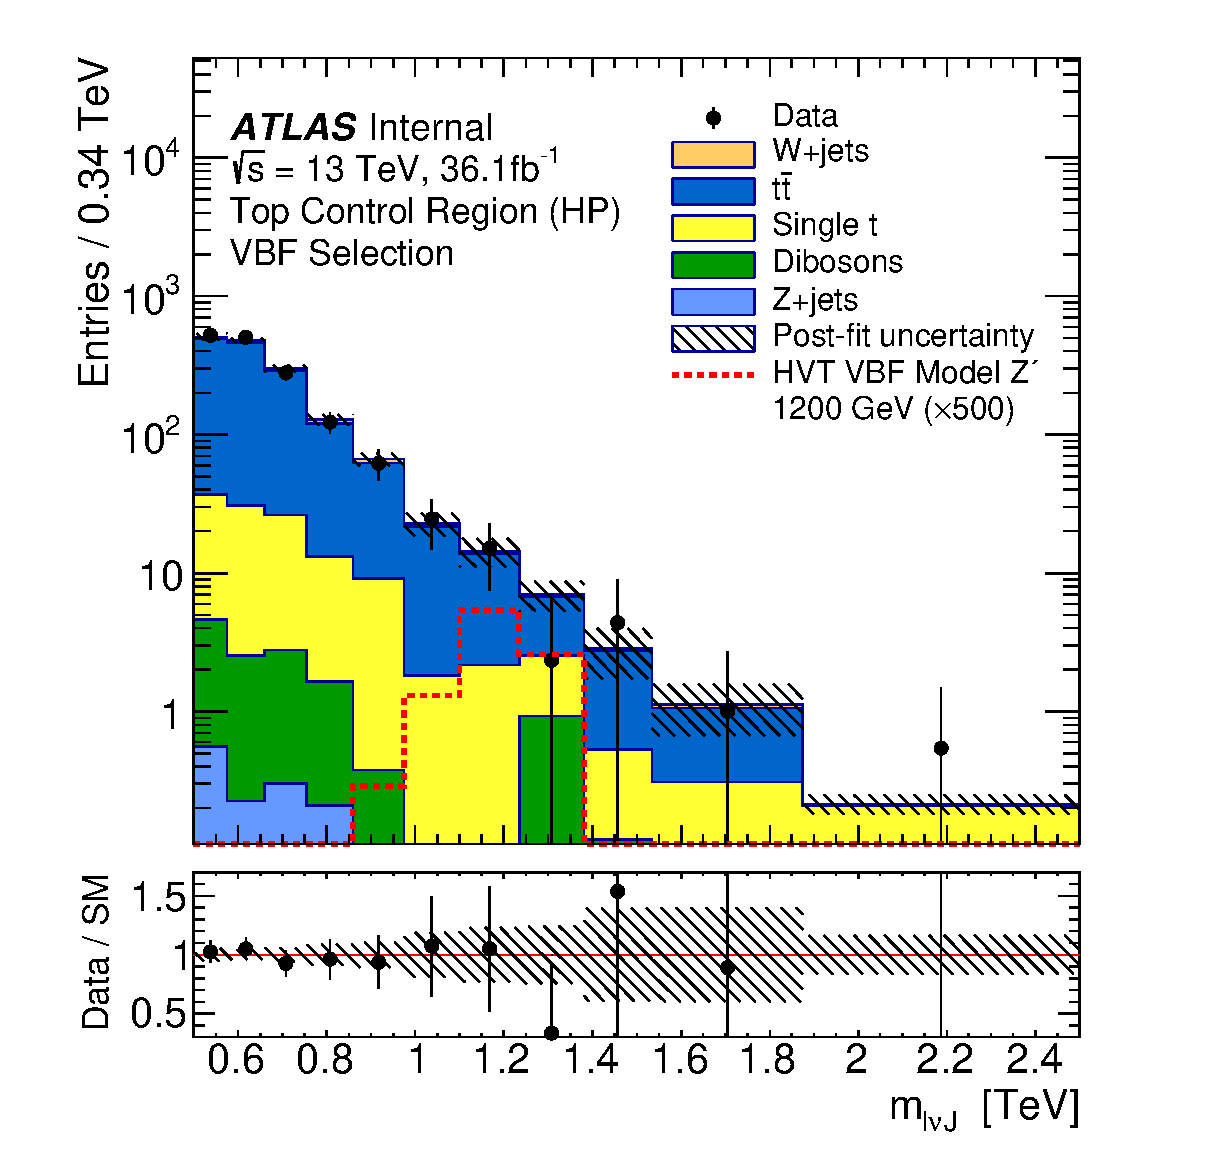
\includegraphics[width=.48\textwidth]{figures/Results/new/final_pf/postFit_VBF_HVTWW_1000_TCR_HP}\label{fig:pf_hp_vbf:d}}
\caption[Post-fit $m(\ell\nu J)$ distribution for high purity, vector boson fusion selection]{The post-fit $m(\ell\nu J)$ distributions for the HP VBF selection in \protect\subref{fig:pf_hp_vbf:a} the $WW$ SR, \protect\subref{fig:pf_hp_vbf:b} the $WZ$ SR, \protect\subref{fig:pf_hp_vbf:c} the \Wjets CR, and   \protect\subref{fig:pf_hp_vbf:d} the \ttbar CR. The pre-fit HVT (VBF production) signal prediction for $m=1.2\,\TeV$\, is overlaid. The shaded band denotes the total post-fit statistical and systematic uncertainty on the background. The ratio of the observed data to SM background prediction is shown in the lower panel. All overflow events are included in the final bin. }
\label{fig:pf_hp_vbf}
\end{figure}

\begin{figure}[htb]
\centering
\subfloat[]{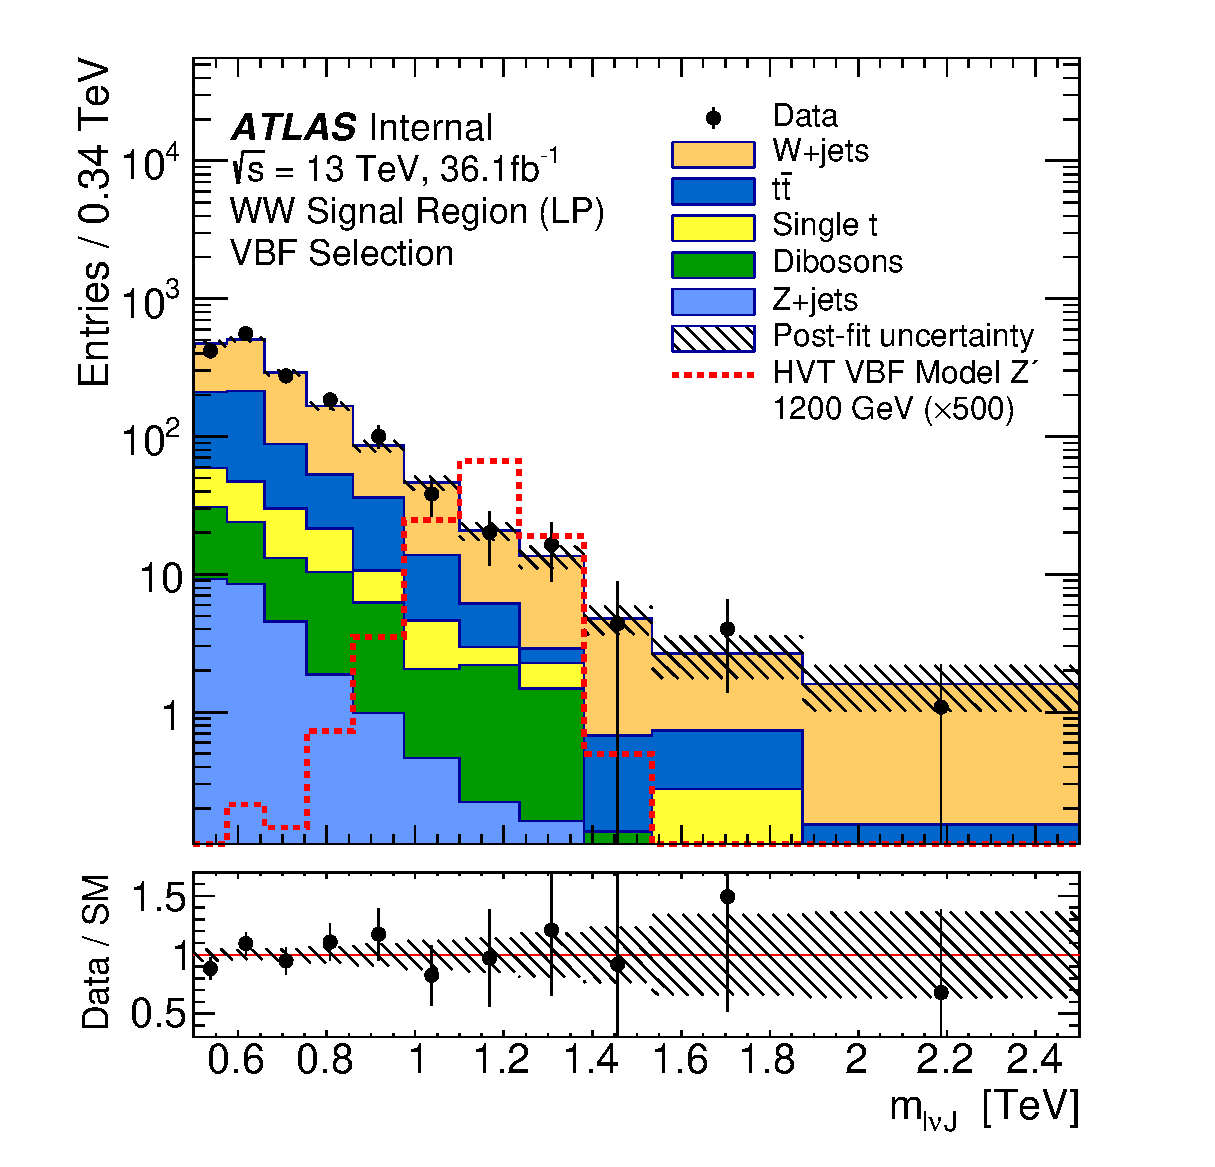
\includegraphics[width=.48\textwidth]{figures/Results/new/final_pf/postFit_VBF_HVTWW_1000_SRWW_LP}\label{fig:pf_lp_vbf:a}}
\subfloat[]{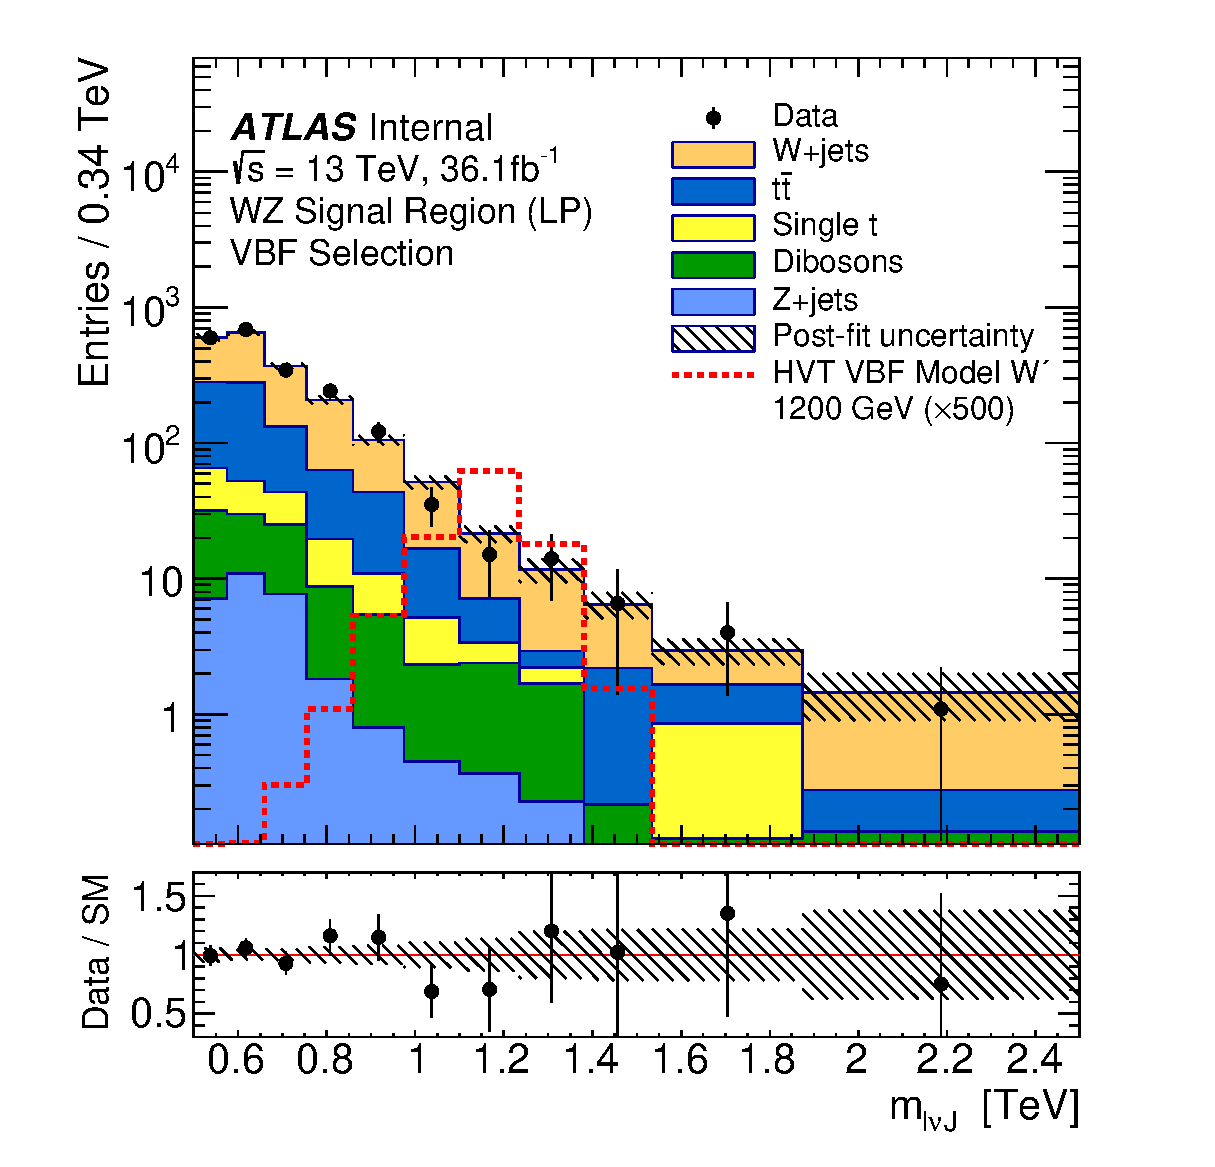
\includegraphics[width=.48\textwidth]{figures/Results/new/final_pf/postFit_VBF_HVTWZ_1000_SRWZ_LP}\label{fig:pf_lp_vbf:b}}\\
\subfloat[]{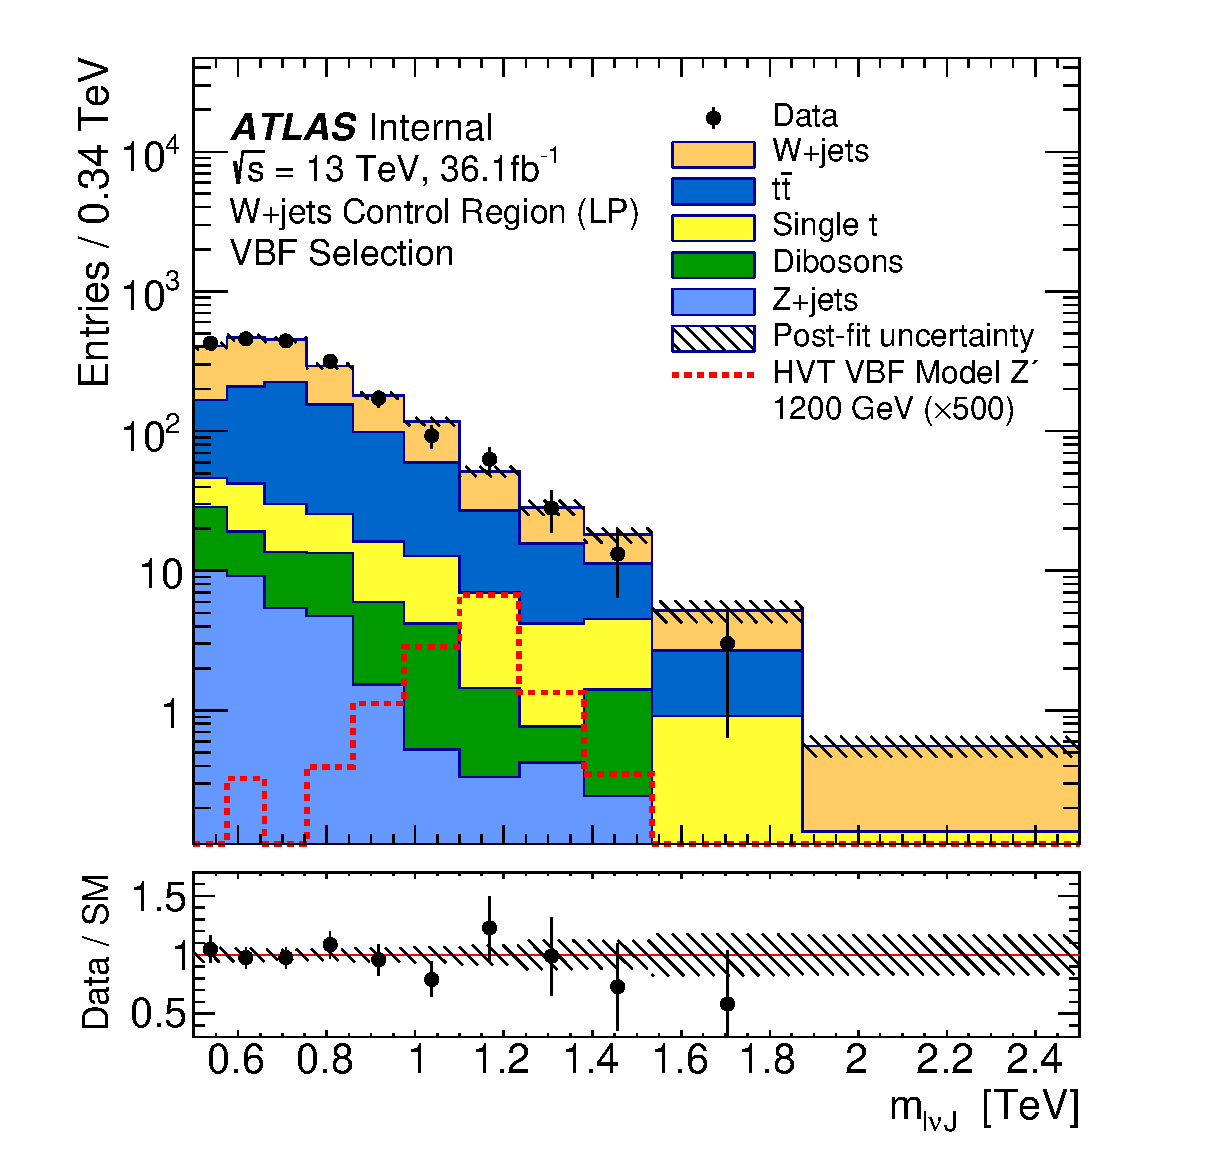
\includegraphics[width=.48\textwidth]{figures/Results/new/final_pf/postFit_VBF_HVTWW_1000_WCR_LP}\label{fig:pf_lp_vbf:c}}
\subfloat[]{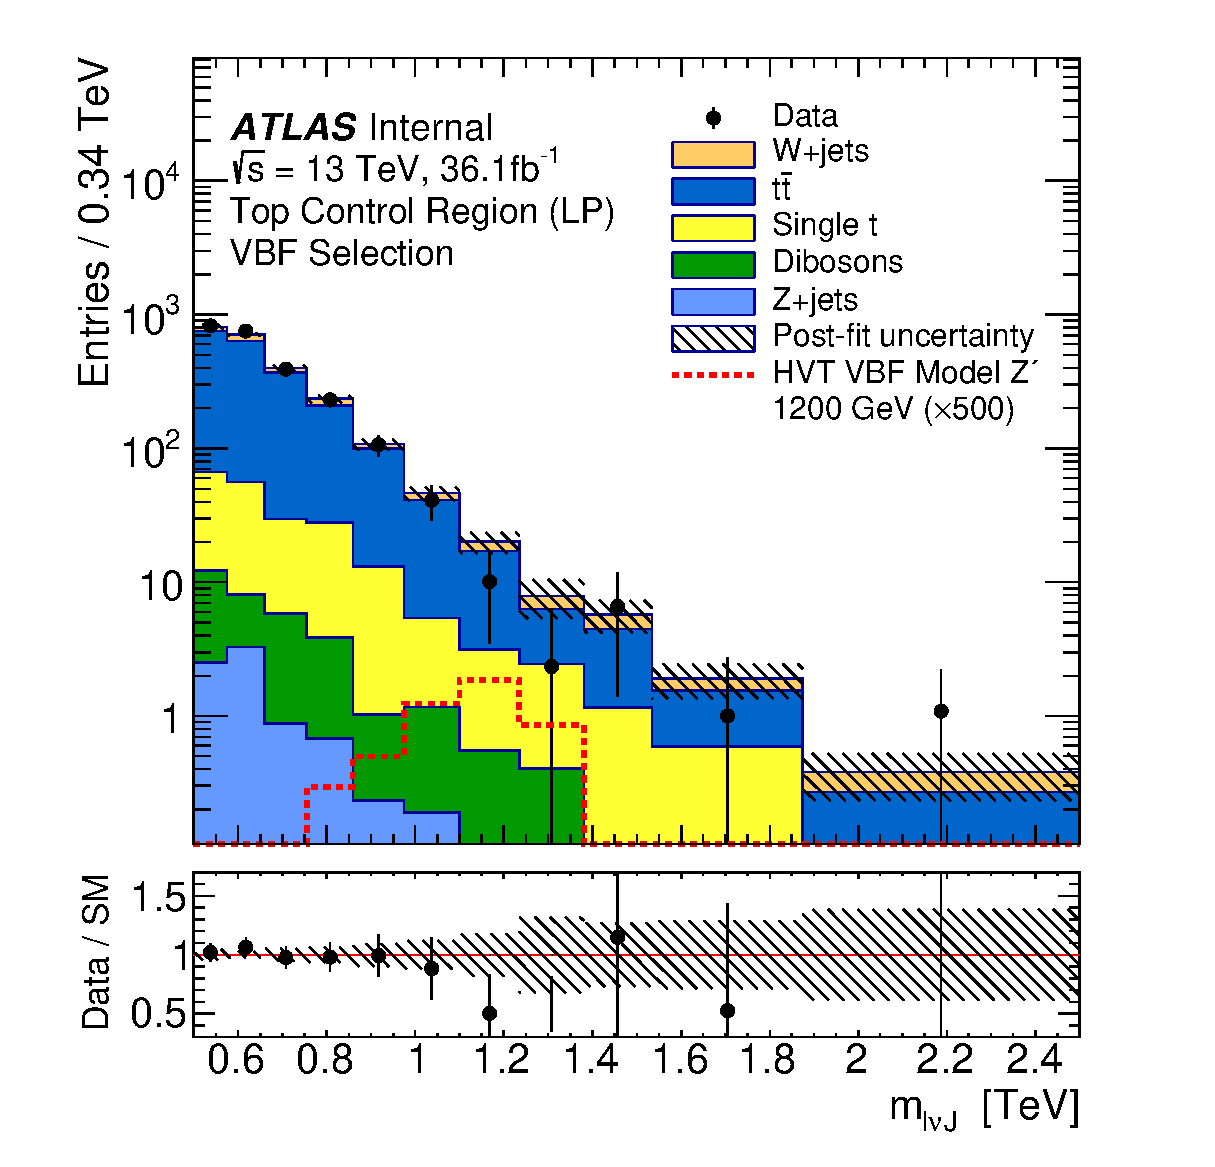
\includegraphics[width=.48\textwidth]{figures/Results/new/final_pf/postFit_VBF_HVTWW_1000_TCR_LP}\label{fig:pf_lp_vbf:d}}
\caption[Post-fit $m(\ell\nu J)$ distribution for low purity, vector boson fusion selection]{The post-fit $m(\ell\nu J)$ distributions for the LP VBF selection in \protect\subref{fig:pf_lp_vbf:a} the $WW$ SR, \protect\subref{fig:pf_lp_vbf:b} the $WZ$ SR, \protect\subref{fig:pf_lp_vbf:c} the \Wjets CR, and   \protect\subref{fig:pf_lp_vbf:d} the \ttbar CR.  The pre-fit HVT (VBF production) signal prediction for $m=1.2\,\TeV$\, is overlaid. The shaded band denotes the total post-fit statistical and systematic uncertainty on the background. The ratio of the observed data to SM background prediction is shown in the lower panel. All overflow events are included in the final bin.}
\label{fig:pf_lp_vbf}
\end{figure}

\begin{figure}[htb]
\centering
\subfloat[]{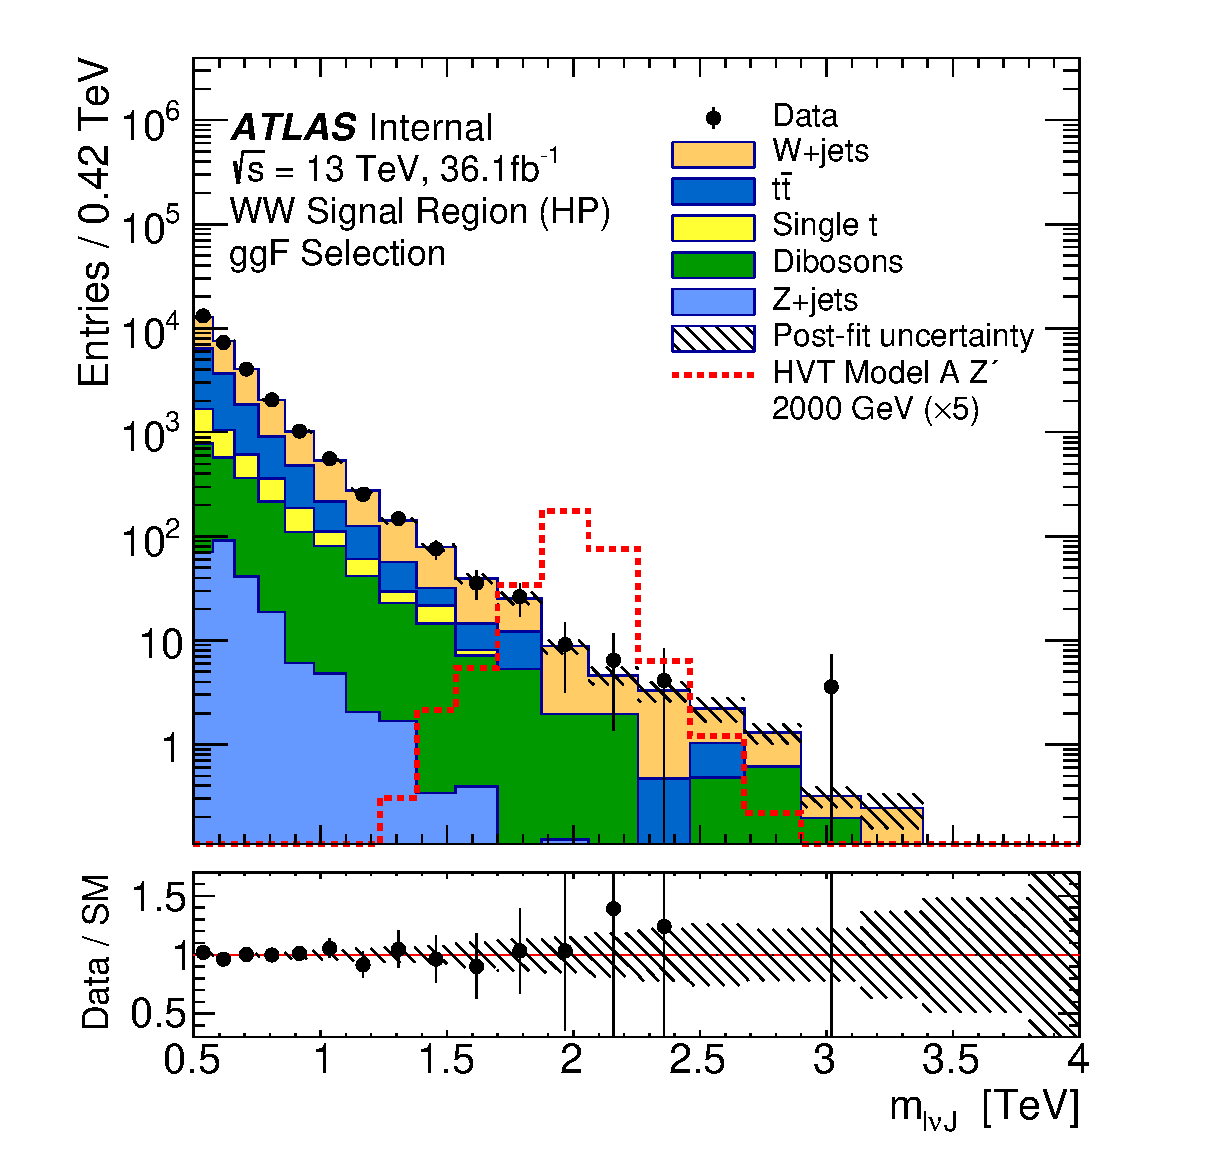
\includegraphics[width=.48\textwidth]{figures/Results/new/final_pf/postFit_HVTWW_2000_SRWW_HP}\label{fig:pf_hp_ggf:a}}
\subfloat[]{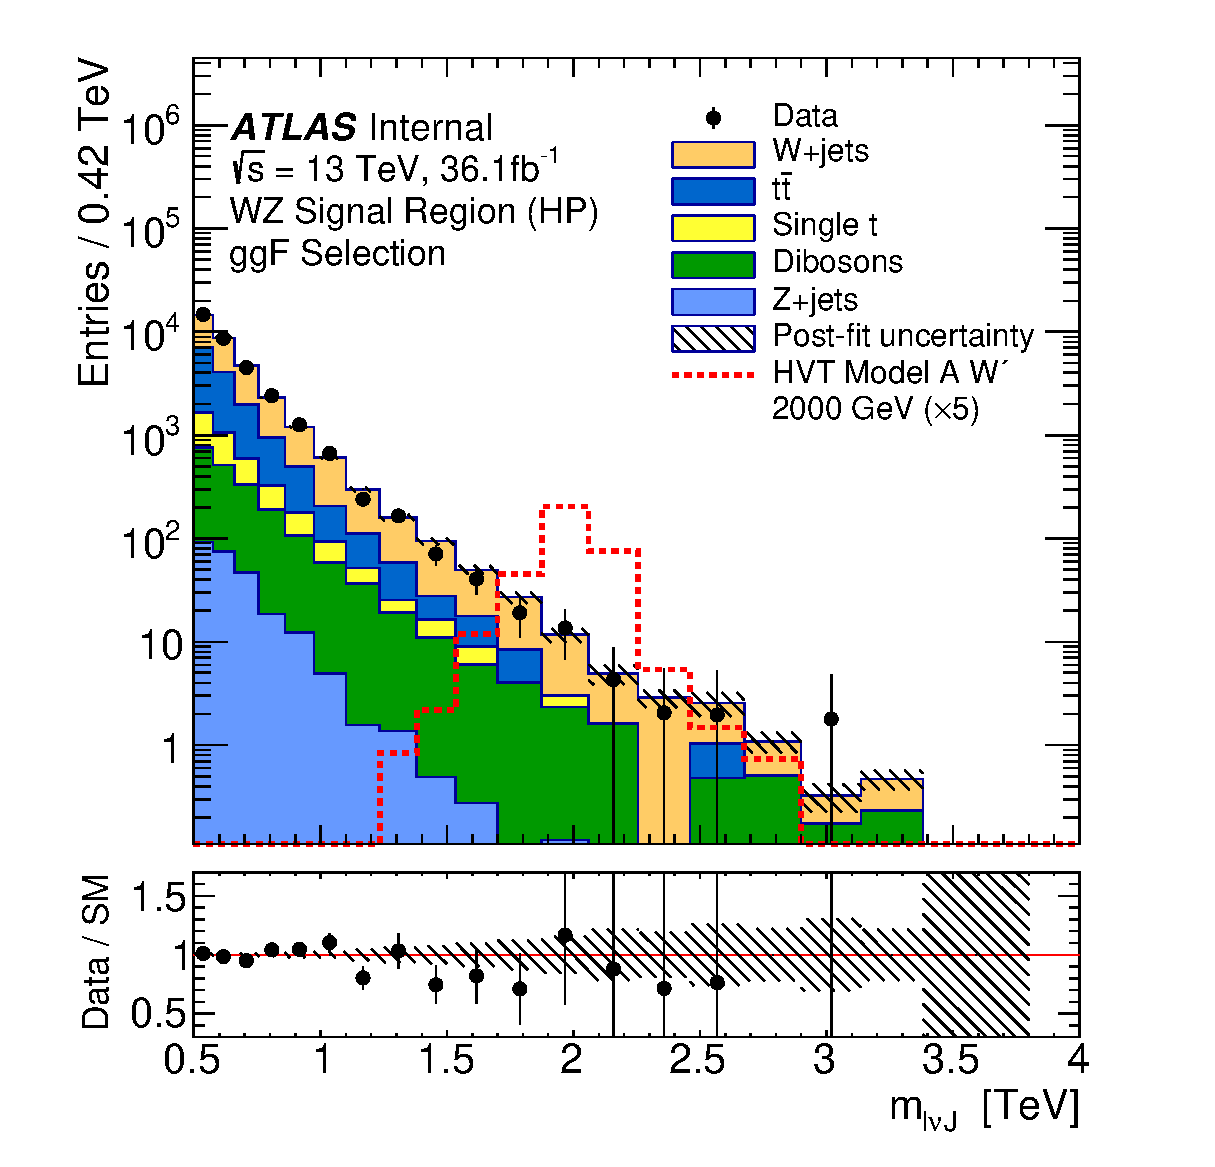
\includegraphics[width=.48\textwidth]{figures/Results/new/final_pf/postFit_HVTWZ_2000_SRWZ_HP}\label{fig:pf_hp_ggf:b}}\\
\subfloat[]{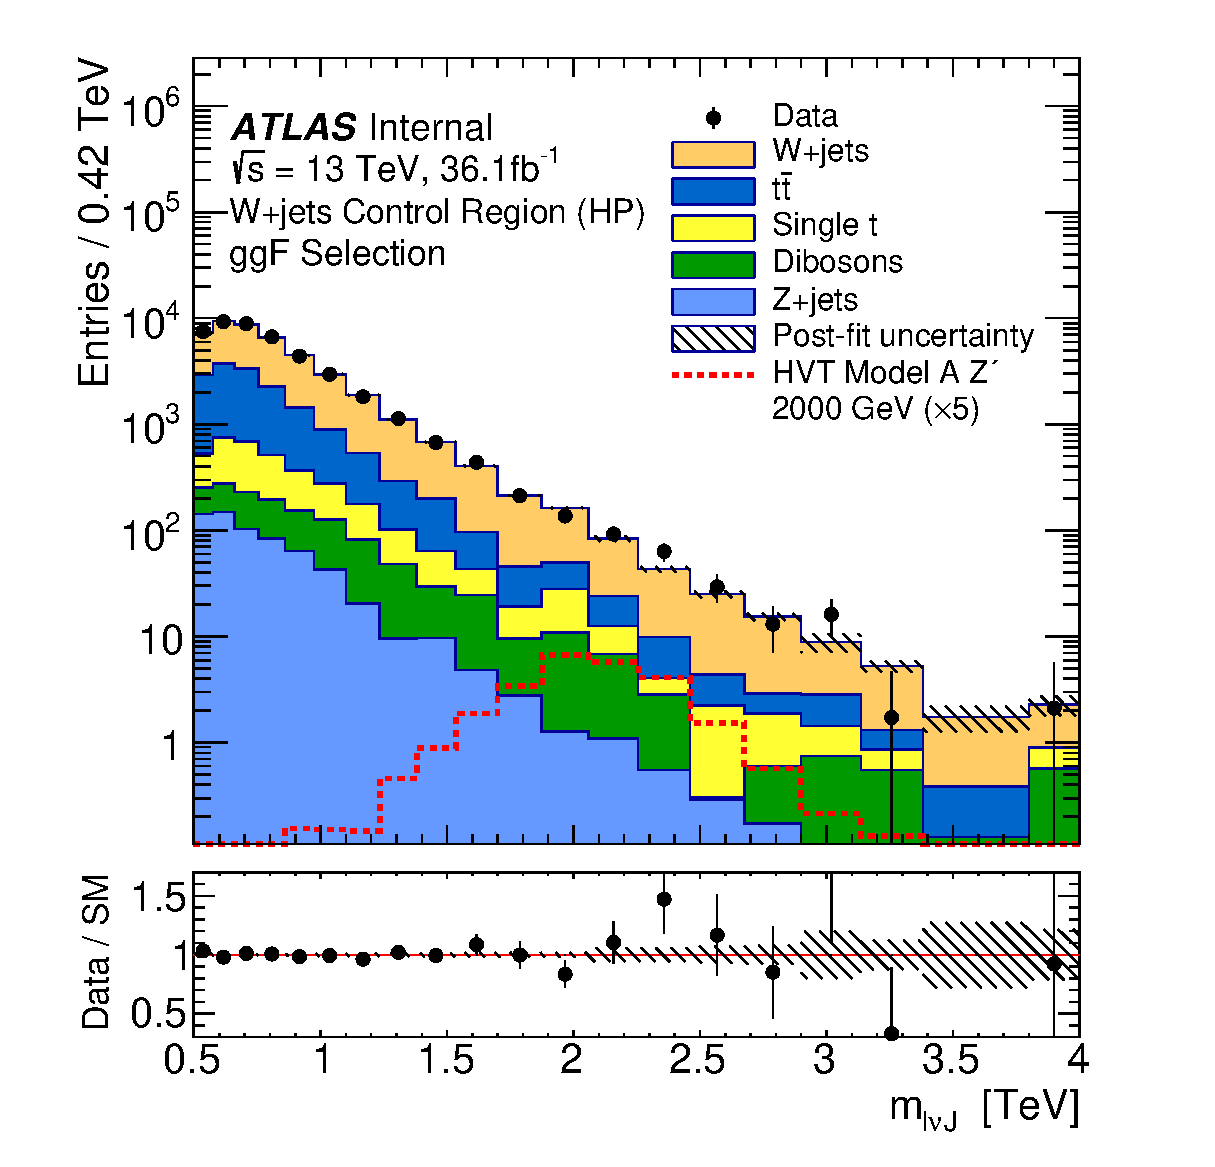
\includegraphics[width=.48\textwidth]{figures/Results/new/final_pf/postFit_HVTWW_2000_WCR_HP}\label{fig:pf_hp_ggf:c}}
\subfloat[]{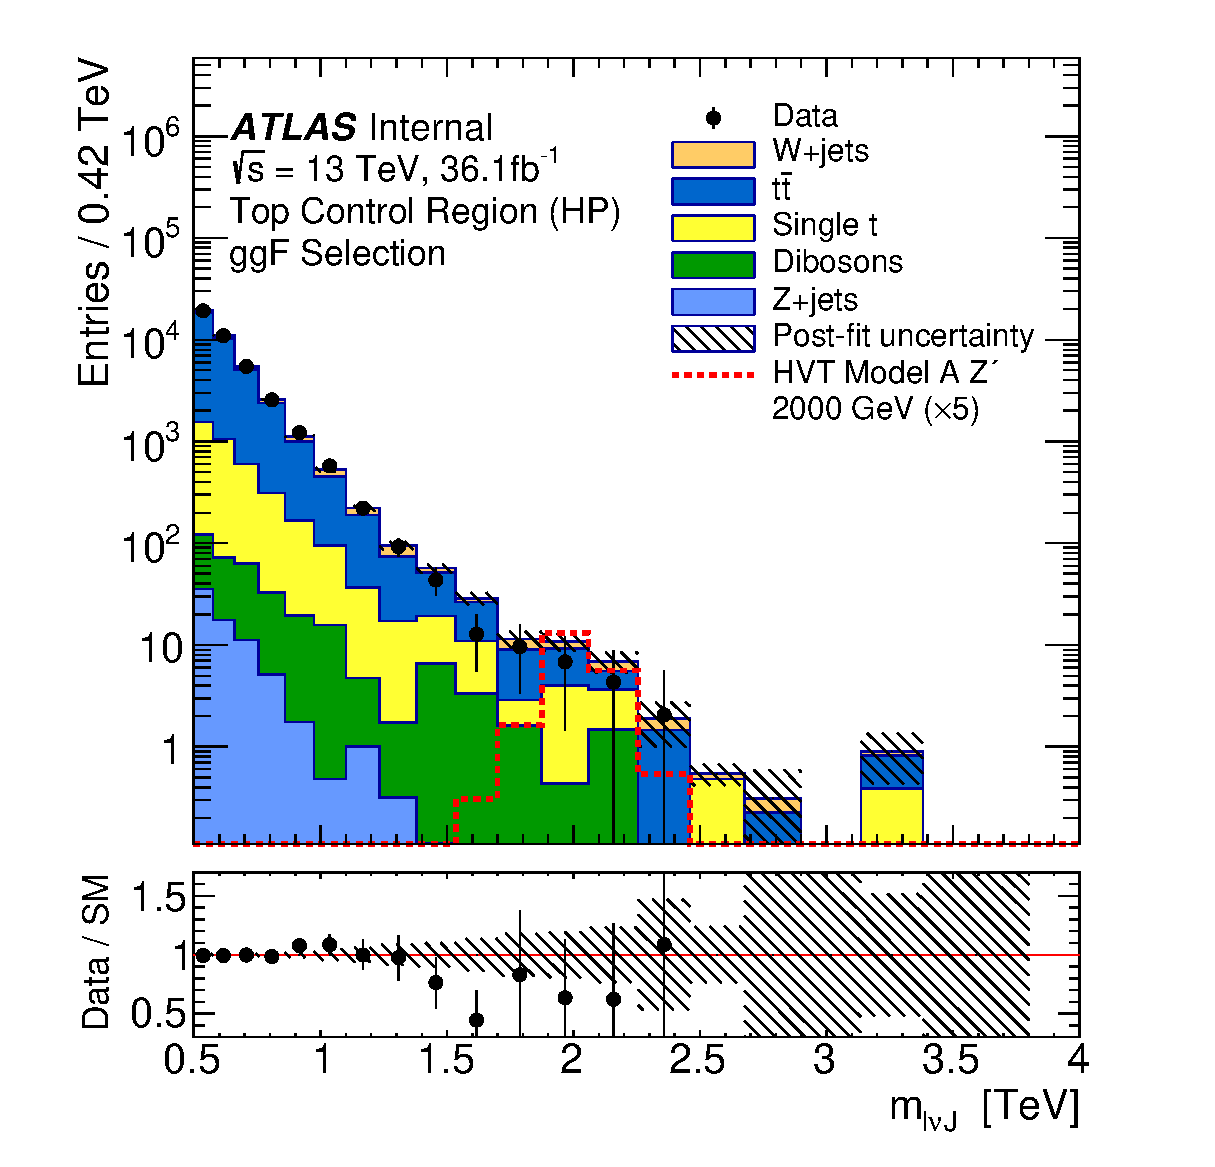
\includegraphics[width=.48\textwidth]{figures/Results/new/final_pf/postFit_HVTWW_2000_TCR_HP}\label{fig:pf_hp_ggf:d}}
\caption[Post-fit $m(\ell\nu J)$ distribution for high purity, gluon-gluon fusion selection]{The post-fit $m(\ell\nu J)$ distributions for the HP ggF selection in \protect\subref{fig:pf_hp_ggf:a} the $WW$ SR, \protect\subref{fig:pf_hp_ggf:b} the $WZ$ SR, \protect\subref{fig:pf_hp_ggf:c} the \Wjets CR, and   \protect\subref{fig:pf_hp_ggf:d} the \ttbar CR. The pre-fit HVT (qqF production) signal prediction for $m=2.0\,\TeV$\, is overlaid. The shaded band denotes the total post-fit statistical and systematic uncertainty on the background. The ratio of the observed data to SM background prediction is shown in the lower panel. All overflow events are included in the final bin.}
\label{fig:pf_hp_ggf}
\end{figure}

\begin{figure}[htb]
\centering
\subfloat[]{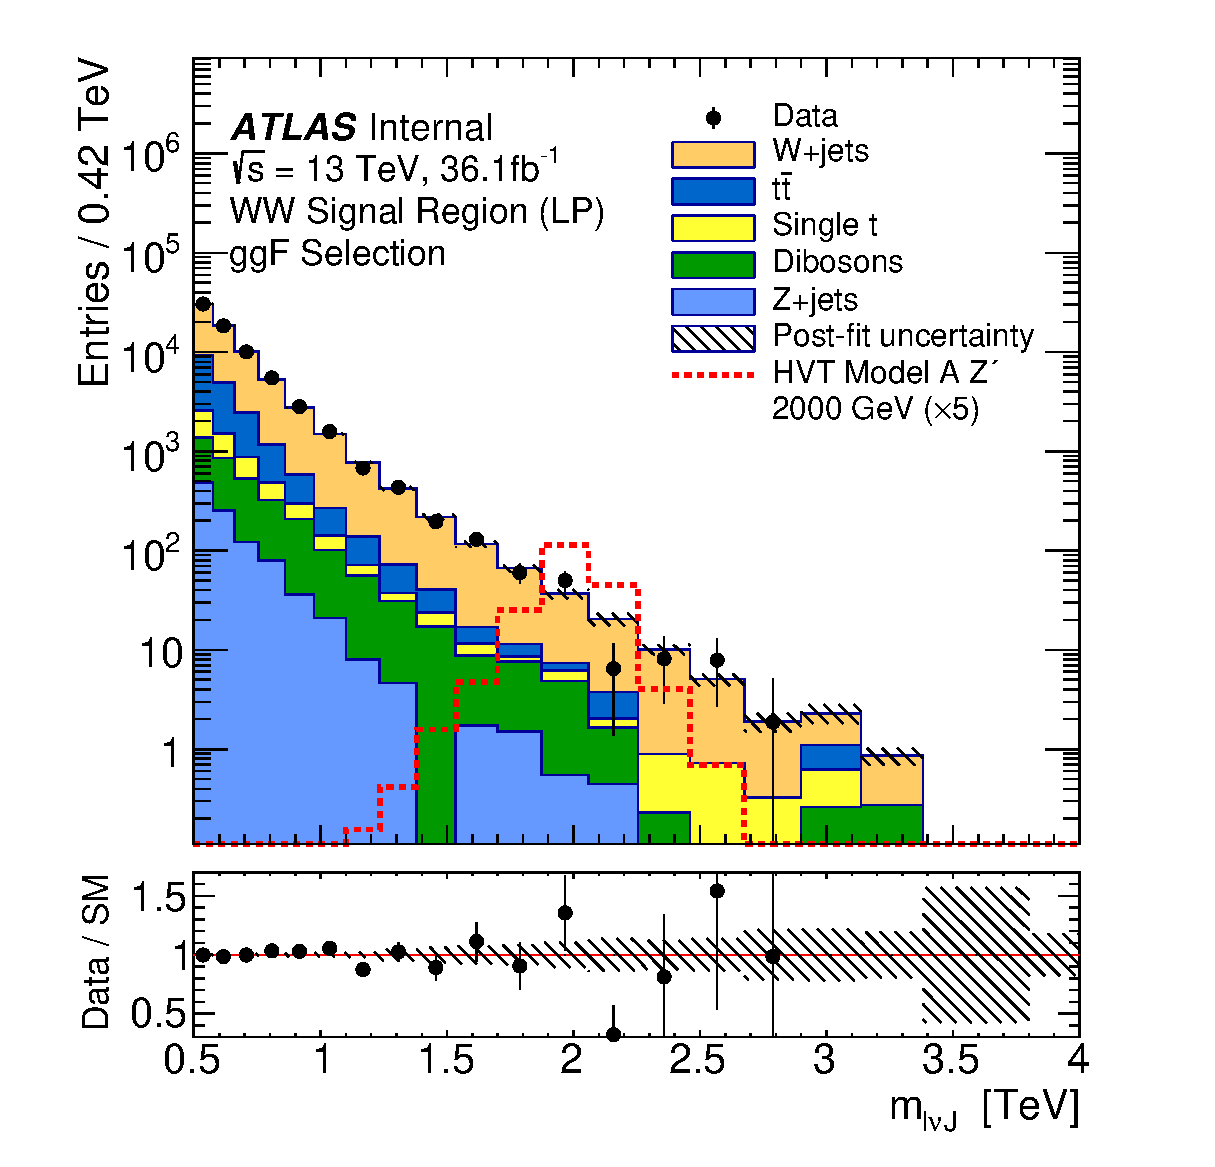
\includegraphics[width=.48\textwidth]{figures/Results/new/final_pf/postFit_HVTWW_2000_SRWW_LP}\label{fig:pf_lp_ggf:a}}
\subfloat[]{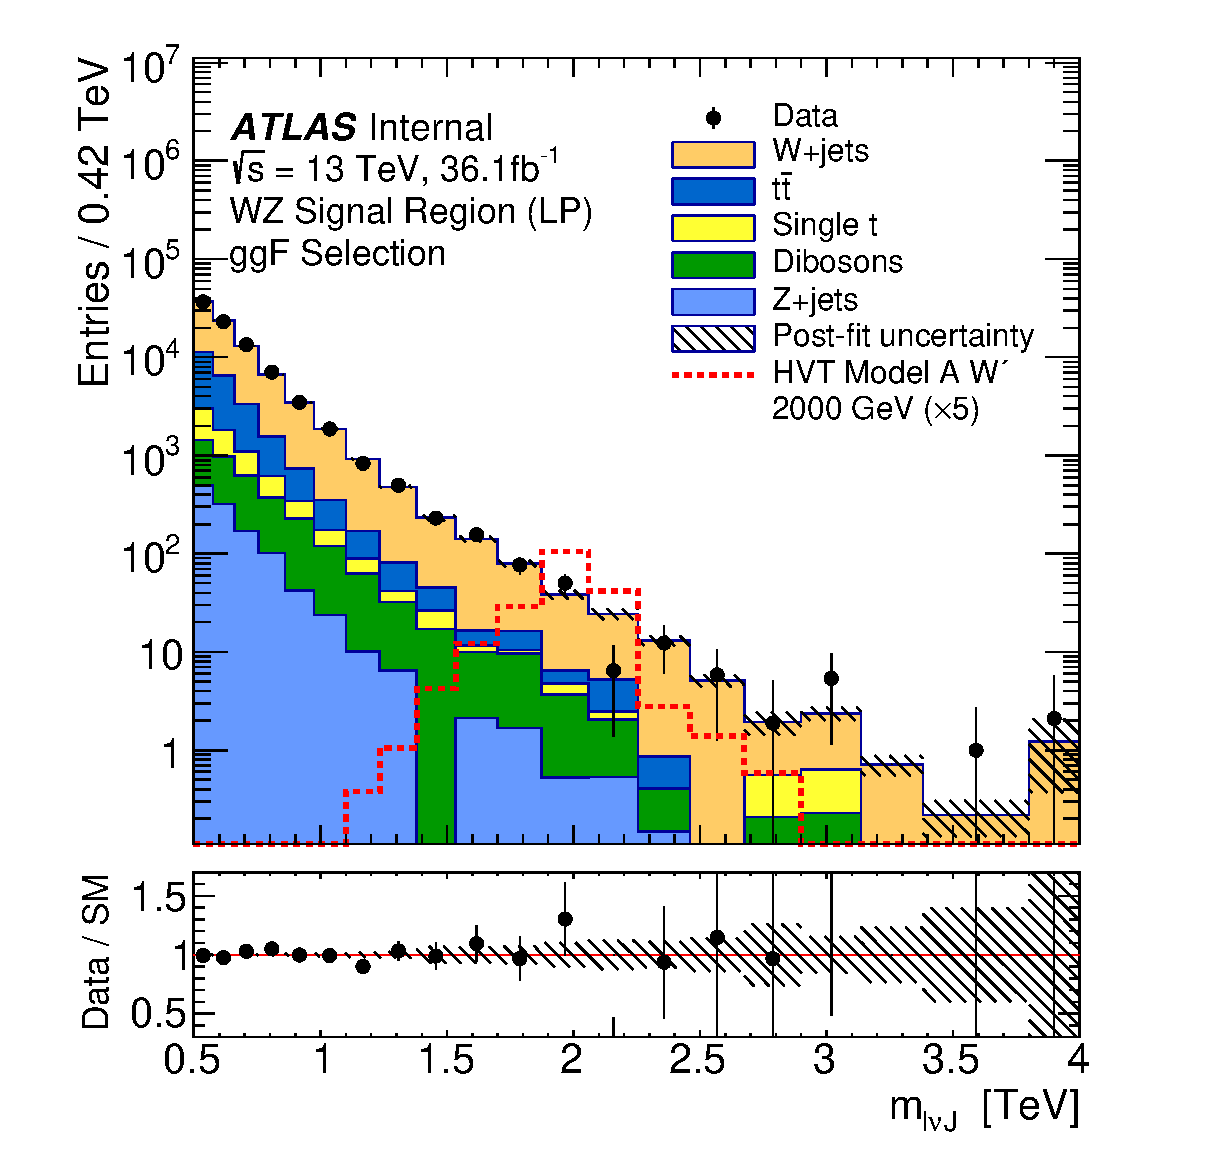
\includegraphics[width=.48\textwidth]{figures/Results/new/final_pf/postFit_HVTWZ_2000_SRWZ_LP}\label{fig:pf_lp_ggf:b}}\\
\subfloat[]{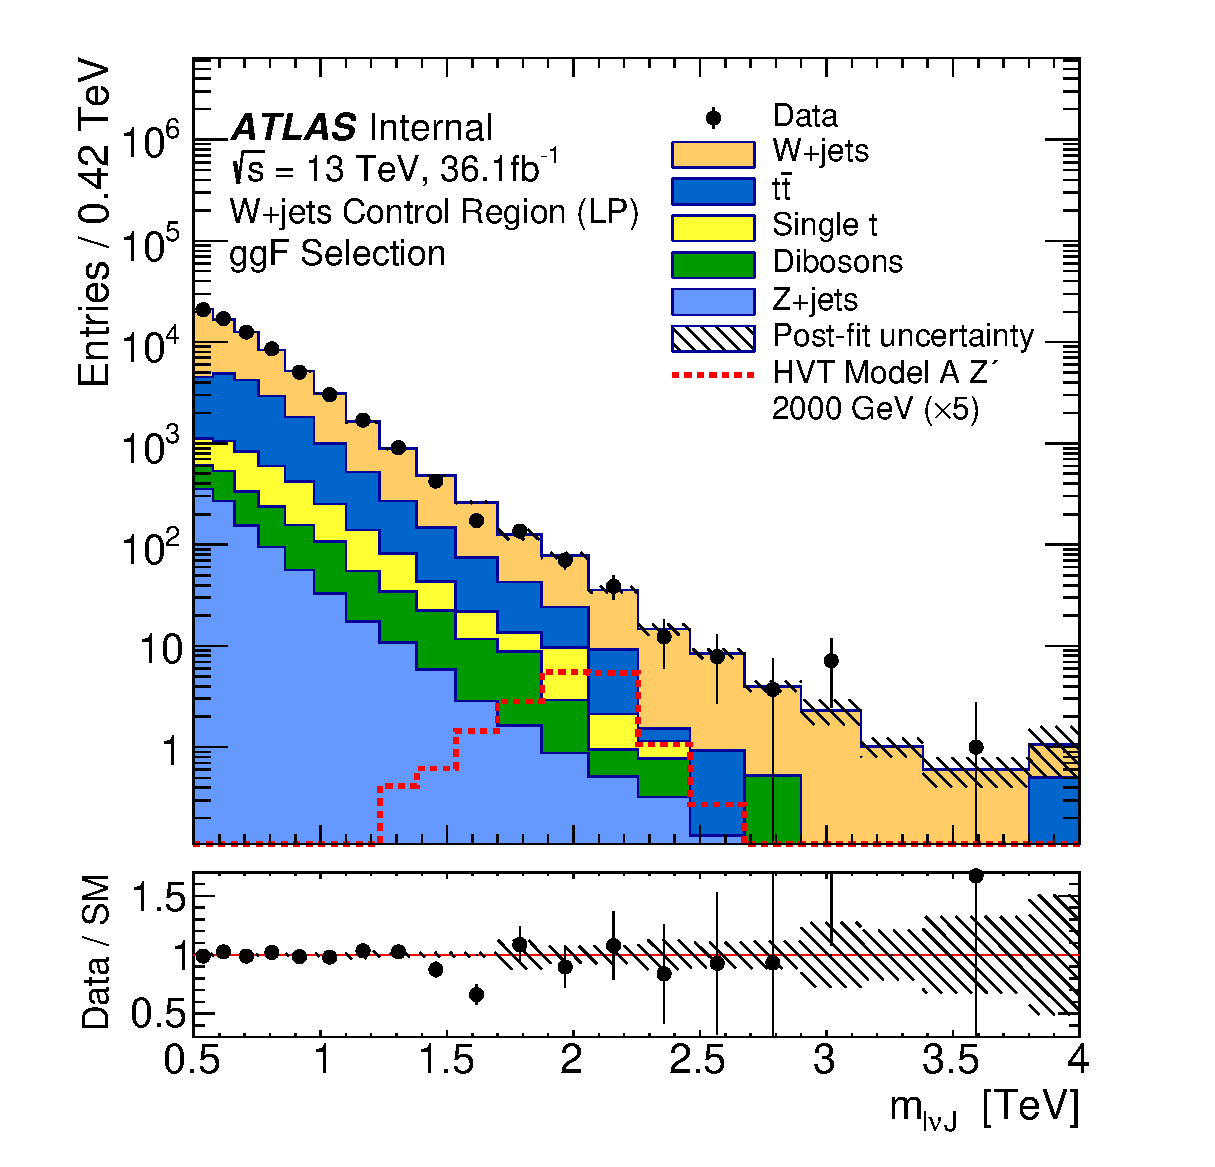
\includegraphics[width=.48\textwidth]{figures/Results/new/final_pf/postFit_HVTWW_2000_WCR_LP}\label{fig:pf_lp_ggf:c}}
\subfloat[]{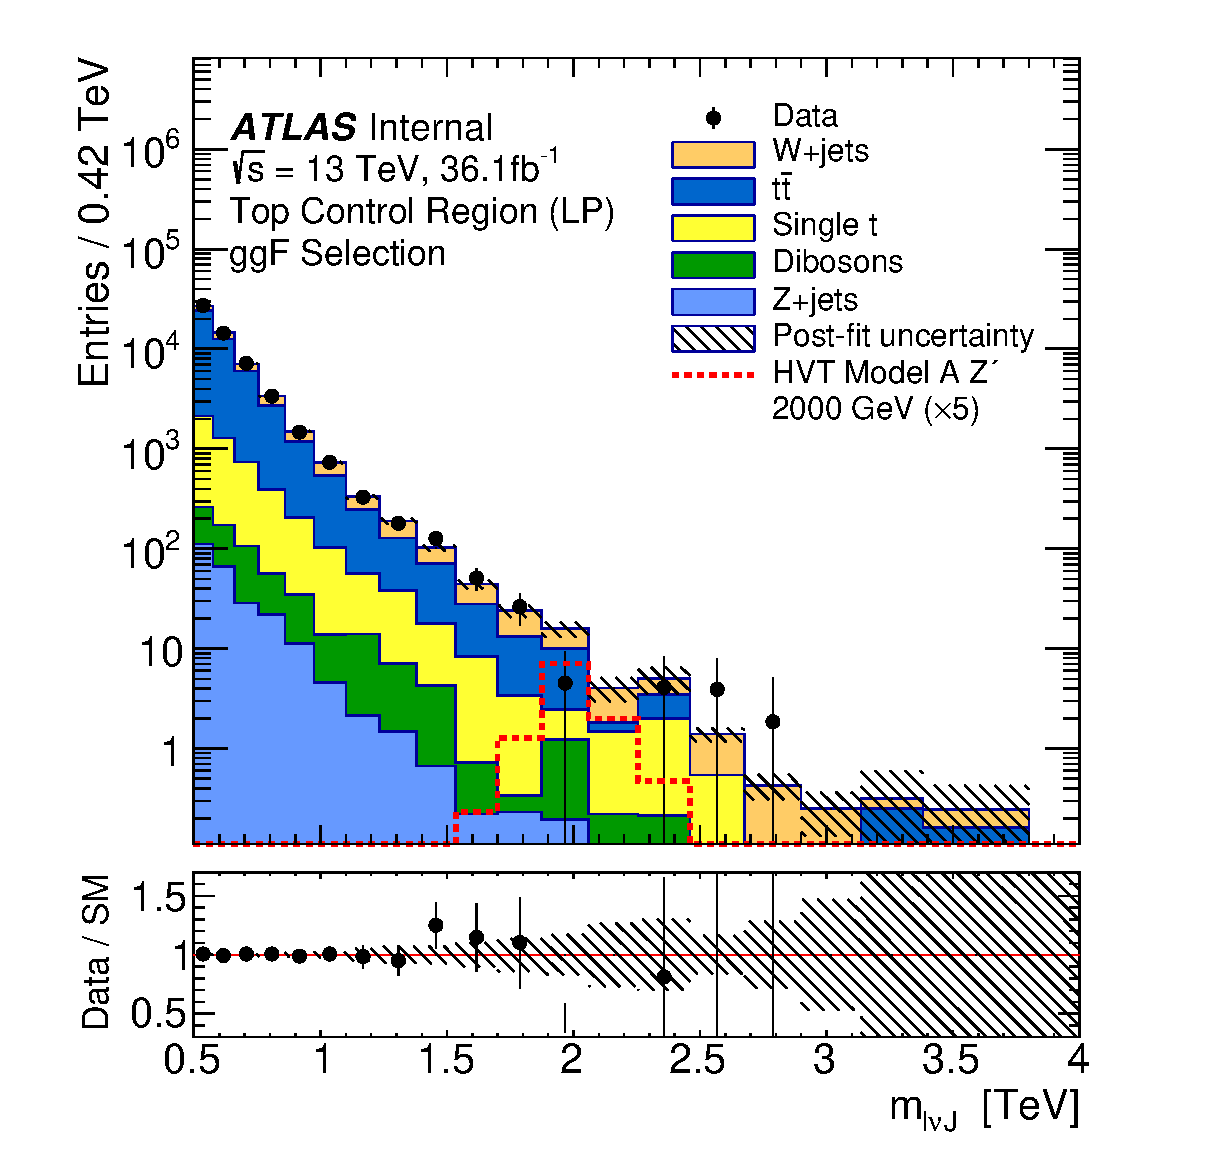
\includegraphics[width=.48\textwidth]{figures/Results/new/final_pf/postFit_HVTWW_2000_TCR_LP}\label{fig:pf_lp_ggf:d}}
\caption[Post-fit $m(\ell\nu J)$ distribution for low purity, gluon-gluon fusion selection]{The post-fit $m(\ell\nu J)$ distributions for the LP ggF selection in \protect\subref{fig:pf_lp_ggf:a} the $WW$ SR, \protect\subref{fig:pf_lp_ggf:b} the $WZ$ SR, \protect\subref{fig:pf_lp_ggf:c} the \Wjets CR, and   \protect\subref{fig:pf_lp_ggf:d} the \ttbar CR. The pre-fit HVT (qqF production) signal prediction for $m=2.0\,\TeV$\, is overlaid. The shaded band denotes the total post-fit statistical and systematic uncertainty on the background. The ratio of the observed data to SM background prediction is shown in the lower panel. All overflow events are included in the final bin.}
\label{fig:pf_lp_ggf}
\end{figure}

\clearpage
Across all SRs and CRs, the fitted background distributions agree well with the observed data distributions, within the total estimated uncertainty. The shape of the $m(\ell\nu J)$ distribution is modeled well, with no apparent trends in the ratio plots in the lower panels. 
%Several bins show small fluctuations outside the estimated uncertainty bands; however, these fluctuations are mostly accompanied by nearby fluctuations in the opposite direction. 
The strong agreement in the CRs, where no signal leak is expected, lends confidence to the estimation and modeling of the two principal backgrounds, \Wjets and \ttbar. 


The \Wjets and \ttbar normalization factors, defined as the ratio of the number of simulated events after the fit to the number of simulated events before the fit, are shown in~\Tab{\ref{tab:bkg_norms}}. The values were constrained by the simultaneous fit to the SRs and dedicated CRs, but allowed to float. Fitted normalization factors close to unity indicate accurate modeling of the cross sections of the respective background processes.  All normalization factors are consistent with unity, within approximately one standard deviation of the measured value. The uncertainty on the normalization factor includes statistical and systematic uncertainties.

For each of the four fits, the event yields for the observed data and the post-fit simulated SM backgrounds are calculated for the HP SR and CRs, and the LP SR and CRs. In~\Tab{\ref{tab:yields_VBFWW}}, the event yields are shown for the $WW$ and $WZ$ channel fits, with VBF selection. In~\Tab{\ref{tab:yields_WW}}, the event yields are shown for the $WW$ and $WZ$ channel fits, with ggF selection. The numbers of observed data events are listed without uncertainty. The SM background event yields include statistical and systematic uncertainties. Event yields for each individual background process, and the total background prediction, are included. Correlations between the SM backgrounds are taken into account; therefore, the quoted uncertainty for the total background prediction does not necessarily correspond to the sum in quadrature of each individual background uncertainty. For each region, the observed number of data events matches the total SM prediction within the estimated uncertainty. 

% Normalization factors
\begin{table}[tb]
\centering
\caption[Normalization factors for the \Wjets and $\ttbar$ backgrounds]{Normalization factors for the \Wjets and \ttbar backgrounds for the $WW$ and $WZ$ channels, separated into ggF and VBF selections. The normalization factor is the ratio between the number of fitted events from simulation to the number of predicted events from simulation. The uncertainties include both statistical and systematic uncertainties.}
\begin{tabular}{r|cc|cc}
\hline\hline
Bkg. & \multicolumn{2}{c|}{$WW$ Selection} & \multicolumn{2}{c}{$WZ$ Selection}\\\cline{2-5}
Norm. & ggF & VBF & ggF & VBF \\\hline
\Wjets&$0.95\pm0.06$&$0.89\pm0.18$&$0.97\pm0.06$&$0.84\pm0.16$\\\hline
\ttbar&$1.03\pm0.06$&$1.21\pm0.18$&$1.00\pm0.06$&$1.10\pm0.17$\\\hline\hline
\end{tabular}
\label{tab:bkg_norms}
\end{table}

% Yields
\begin{table}[tbp]
\renewcommand{\arraystretch}{1.25}
\caption[Expected and observed event yields (vector boson fusion selection)]{Expected and observed event yields in the signal regions and control regions for the VBF $WW$ and $WZ$ selections.  Yields and uncertainties are evaluated after a background-only fit to the data in all regions indicated above.  The uncertainty on the total background estimate can be smaller than the quadratic sum of the individual background contributions due to anti-correlations between the estimates of different background sources.}
\begin{center}
\resizebox{\textwidth}{!}{%
\begin{tabular}{c | c@{\ $\pm$\ }c c@{\ $\pm$\ }c c@{\ $\pm$\ }c | c@{\ $\pm$\ }c  c@{\ $\pm$\ }c c@{\ $\pm$\ }c}
\hline
\hline
VBF $WW$&\multicolumn{6}{c|}{High Purity}&\multicolumn{6}{c}{Low Purity}\\
\cline{2-13}
Selection&\multicolumn{2}{c}{SR}&\multicolumn{2}{c}{$W$+jets CR}&\multicolumn{2}{c|}{Top CR}&\multicolumn{2}{c}{SR}&\multicolumn{2}{c}{$W$+jets CR}&\multicolumn{2}{c}{Top CR}\\
\hline
$W$+jets&71&15&183&26&18&4&268&31&294&35&55&11\\
$\ttbar$&84&16&179&22&346&19&115&24&225&30&500&27\\
Single-$t$&13&3&24&6&30&5&23&5&31&6&47&9\\
SM Diboson&9.8&3.4&13&4&3.3&1.1&17&6&16&5&6.7&3.2\\
$Z$+jets&1.6&0.5&4.5&0.9&0.5&0.3&6.7&2.1&8.7&2.1&2.0&0.7\\
\hline
Total Background&178&12&403&19&398&18&431&20&573&23&611&23\\
\hline
Observed&\multicolumn{2}{c}{176}&\multicolumn{2}{c}{402}&\multicolumn{2}{c|}{398}&\multicolumn{2}{c}{436}&\multicolumn{2}{c}{567}&\multicolumn{2}{c}{613}\\
\hline
\hline
\end{tabular}
}
\label{tab:yields_VBFWW}
\end{center}
%\end{table}
%
%\begin{table}[tbp]
\renewcommand{\arraystretch}{1.25}
%\caption{Expected and observed yields in signal and control regions for the VBF $WZ$ signal hypothesis.  Yields and uncertainties are evaluated after a background-only fit to the data in all regions indicated above.  The uncertainty on the total background estimate can be smaller than the quadratic sum of the individual background contributions due to anti-correlations between the estimates of different background sources.}
\begin{center}
\resizebox{\textwidth}{!}{%
\begin{tabular}{c | c@{\ $\pm$\ }c c@{\ $\pm$\ }c c@{\ $\pm$\ }c | c@{\ $\pm$\ }c  c@{\ $\pm$\ }c c@{\ $\pm$\ }c}
\hline
\hline
VBF $WZ$&\multicolumn{6}{c|}{High Purity}&\multicolumn{6}{c}{Low Purity}\\
\cline{2-13}
Selection&\multicolumn{2}{c}{SR}&\multicolumn{2}{c}{$W$+jets CR}&\multicolumn{2}{c|}{Top CR}&\multicolumn{2}{c}{SR}&\multicolumn{2}{c}{$W$+jets CR}&\multicolumn{2}{c}{Top CR}\\
\hline
$W$+jets&75&17&187&27&18&5&323&42&302&41&58&12\\
$\ttbar$&106&24&175&45&346&36&161&49&224&56&496&52\\
Single-$t$&12&6&24&10&31&10&26&11&30&9&47&19\\
SM Diboson&10&5&11&5&2.7&1.1&22&10&14&5&5.9&4.1\\
$Z$+jets&1.6&1.5&4.6&2.3&0.4&0.2&7.8&6.0&8.4&3.9&1.9&1.2\\
\hline
Total Background&205&28&402&52&398&41&540&49&578&47&609&66\\
\hline
Observed&\multicolumn{2}{c}{201}&\multicolumn{2}{c}{402}&\multicolumn{2}{c|}{398}&\multicolumn{2}{c}{550}&\multicolumn{2}{c}{567}&\multicolumn{2}{c}{613}\\
\hline
\hline
\end{tabular}
}
\label{tab:yields_VBFWZ}
\end{center}
\end{table}

%\input{figures/Results/new/VBFWZ_yields.tex}
\begin{table}[tbp]
\renewcommand{\arraystretch}{1.25}
\caption[Expected and observed event yields (gluon-gluon fusion selection)]{Expected and observed event yields in the signal regions and control regions for the ggF $WW$ and $WZ$ selections.  Yields and uncertainties are evaluated after a background-only fit to the data in all regions indicated above.  The uncertainty on the total background estimate can be smaller than the quadratic sum of the individual background contributions due to anti-correlations between the estimates of different background sources.}
\begin{center}
\resizebox{\textwidth}{!}{%
\begin{tabular}{c | c@{\ $\pm$\ }c c@{\ $\pm$\ }c c@{\ $\pm$\ }c | c@{\ $\pm$\ }c  c@{\ $\pm$\ }c c@{\ $\pm$\ }c}
\hline
\hline
ggF $WW$&\multicolumn{6}{c|}{High Purity}&\multicolumn{6}{c}{Low Purity}\\
\cline{2-13}
Selection&\multicolumn{2}{c}{SR}&\multicolumn{2}{c}{$W$+jets CR}&\multicolumn{2}{c|}{Top CR}&\multicolumn{2}{c}{SR}&\multicolumn{2}{c}{$W$+jets CR}&\multicolumn{2}{c}{Top CR}\\
\hline
$W$+jets&3116&165&6848&206&540&60&10790&251&10972&255&1424&167\\
$\ttbar$&2043&142&2920&180&6883&138&2648&187&3790&222&8738&235\\
Single-$t$&374&44&487&57&704&84&493&56&553&64&819&97\\
SM Diboson&353&94&167&45&51&14&431&118&201&55&70&20\\
$Z$+jets&49&6&143&17&15&3&205&25&215&27&54&9\\
\hline
Total Background&5935&70&10565&96&8192&87&14566&120&15730&124&11105&104\\
\hline
Observed&\multicolumn{2}{c}{5885}&\multicolumn{2}{c}{10619}&\multicolumn{2}{c|}{8178}&\multicolumn{2}{c}{14566}&\multicolumn{2}{c}{15707}&\multicolumn{2}{c}{11133}\\
\hline
\hline
\end{tabular}
}
\label{tab:yields_WW}
\end{center}
%\end{table}
%\begin{table}[tbp]
\renewcommand{\arraystretch}{1.25}
%\caption{Expected and observed yields in signal and control regions for the $WZ$ signal hypothesis.  Yields and uncertainties are evaluated after a background-only fit to the data in all regions indicated above.  The uncertainty on the total background estimate can be smaller than the quadratic sum of the individual background contributions due to anti-correlations between the estimates of different background sources.}
\begin{center}
\resizebox{\textwidth}{!}{%
\begin{tabular}{c | c@{\ $\pm$\ }c c@{\ $\pm$\ }c c@{\ $\pm$\ }c | c@{\ $\pm$\ }c  c@{\ $\pm$\ }c c@{\ $\pm$\ }c}
\hline
\hline
ggF $WZ$&\multicolumn{6}{c|}{High Purity}&\multicolumn{6}{c}{Low Purity}\\
\cline{2-13}
Selection&\multicolumn{2}{c}{SR}&\multicolumn{2}{c}{$W$+jets CR}&\multicolumn{2}{c|}{Top CR}&\multicolumn{2}{c}{SR}&\multicolumn{2}{c}{$W$+jets CR}&\multicolumn{2}{c}{Top CR}\\
\hline
$W$+jets&3679&173&6958&191&556&61&13356&299&11091&247&1496&173\\
$\ttbar$&2283&146&2812&167&6842&141&3447&233&3681&218&8611&241\\
Single-$t$&410&50&485&57&749&90&655&75&556&65&854&102\\
SM Diboson&356&98&162&44&51&14&498&138&193&53&71&21\\
$Z$+jets&56&7&148&18&15&3&244&31&212&26&55&9\\
\hline
Total Background&6784&76&10564&96&8211&88&18201&136&15733&124&11087&104\\
\hline
Observed&\multicolumn{2}{c}{6751}&\multicolumn{2}{c}{10619}&\multicolumn{2}{c|}{8178}&\multicolumn{2}{c}{18188}&\multicolumn{2}{c}{15707}&\multicolumn{2}{c}{11133}\\
\hline
\hline
\end{tabular}
}
\label{tab:yields_WZ}
\end{center}
\end{table}

%\input{figures/Results/new/WZ_yields.tex}


%%
\clearpage
\section{Expected and Observed Upper Limits} 
\label{sec:limits}

With no significant excesses above the SM background prediction observed, the fit is performed again with the signal plus background hypothesis (signal with strength $\mu$ not fixed at zero). In~\Tab{\ref{tab:NPranks}}, the top five systematic uncertainties after the fit are listed. The dominant systematic uncertainties for the ggF (VBF) selection are evaluated for the fit performed with the 2\,\TeV\, (1.2\,\TeV) signal mass hypothesis, where the search has a high sensitivity. Additionally, the contributions to the total uncertainty from data statistics and total systematic uncertainties are provided. The uncertainty from data statistics is estimated using a conditional fit, with all the NPs fixed to their best-fit values, $\hat{\theta}$.
%, while the total uncertainty on the signal strength, $\Delta\mu_{\rm tot}$, is estimated from the unconstrained fit where all NPs are floated. 
%The uncertainties listed for each NP, $\Delta\hat{\mu}$, represent the uncertainty on the best-fit signal strength when all the NPs are floated, except the NP in question which is fixed to it's best-fit value.
%, subtracted in quadrature from the total uncertainty: $\Delta\mu_{NP}=\sqrt{(\Delta\mu_{\rm tot})^2-(\Delta\mu_{\rm tot}^{NP {\rm\, fixed}})}$. 
The impact on signal strength is calculated by fixing only the selected NP at its best-fit value, $\hat{\theta}$, and then performing the fit again.
%, varying the NP by its post-fit uncertainty, $\pm\sigma_{\hat{\theta}}$. 
The change in the signal strength from its best-fit value is denoted $\Delta\hat{\mu}$, and indicates how sensitive the signal strength is to the specified NP.

Data statistics are a dominant source of uncertainty in the high mass region, while in the lower mass region, systematic uncertainties related to large-R jet kinematics dominate.  Most of the leading systematic uncertainties are due to modeling of the \Wjets and \ttbar backgrounds.  The relatively conservative uncertainty placed on the SM diboson cross section increases its impact on the signal strength uncertainty.   
The systematic uncertainties related to the large-R jet mass resolution and $D_2^{\beta=1}$ resolution also have significant contributions. As discussed in~\Sect{\ref{ch:syst:largerjets}}, both of these systematic uncertainties have a conservative estimation. 
%For the VBF selection, the \ttbar background comprises a larger percentage of the total SM background with respect to the ggF selection. Consequently, the sensitivity of the signal strength to $b$-tagging increases in this region.

% Systematic uncertainty impact
\begin{table}[tb]
\centering
\caption[Leading systematic uncertainties after the combined fit]{Relative change in signal strength ($\Delta \hat{\mu}$) with respect to the best-fit value after the fit to data. The five dominant uncertainty sources are presented for the ggF and VBF selections, along with the effect of the data statistical uncertainties. These are evaluated from the 2\,\TeV\, (1.2\,\TeV) mass point for the ggF (VBF) selection. To evaluate the impact on $\mu$, the production cross section is assumed the be the expected upper limit at the mass point.}
\vspace{7pt}
\label{tab:NPranks}
\resizebox{\textwidth}{!}{%
\begin{tabular}{cc|cc}
\hline
\hline
 %\multicolumn{2}{c|}{ggF Selection (Fractional uncertainties)} &  \multicolumn{2}{c}{VBF Selection (Fractional uncertainties)} \\
%\hline
%Source & $\Delta \mu_{\rm NP} / \Delta \mu_{\rm total}$ (\%) & Source & $\Delta \mu_{\rm NP} / \Delta \mu_{\rm total}$ (\%) \\
%& $m(WZ) =$  2000 \GeV&  &  $m(WW) =$ 1200 \GeV \\
%\hline
%Simulation statistics              & 28  & Simulation statistics              & 34 \\
%$W$+jets modeling \textsc{MadGraph}& 20  & \Wjets PDF          & 12 \\
%$W$+jets normalization             & 13  & \Wjets $\alpha_s$       & 9 \\
%SM diboson normalization           & 11  & \Wjets normalization    & 9 \\
%$W$+jets modeling scale             & 8   & Top modeling radiation                 & 7 \\
%Top modeling \textsc{MC@NLO}             & 8   & $b$-tagging                        & 7 \\
%\hline
%Total systematic uncertainties     & 41  & Total systematic uncertainties     & 45 \\
%Data statistics                    & 91  & Data statistics                    & 89 \\
%\hline\hline
 %\multicolumn{4}{c}{}\\
 %\multicolumn{4}{c}{}\\
%\hline\hline
 \multicolumn{2}{c|}{ggF Selection (Impact on $\mu$)} &  \multicolumn{2}{c}{VBF Selection (Impact on $\mu$)} \\\hline
%Source & $\Delta \mu_{\rm NP} / \mu$ (\%) & Source & $\Delta \mu_{\rm NP} / \mu$ (\%) \\
Source & $\Delta \hat{\mu} / \mu$ (\%) & Source & $\Delta \hat{\mu} / \mu$ (\%) \\
& $m(WZ) =$  2000 \GeV&  &  $m(WW) =$ 1200 \GeV \\
\hline
$W$+jets modeling \textsc{MadGraph} &  8 & Large-$R$ jets mass resolution           & 5 \\
$W$+jets modeling scale               &  5 & \Wjets PDF                        & 5 \\
SM diboson normalization            &  4 & Top modeling \textsc{Herwig}            & 5 \\
Large-$R$ jets mass resolution      &  4 & $W$+jets normalization & 5 \\
Large-$R$ jets D$_{2}$ resolution   &  4 & Top modeling radiation                  &  4 \\
\hline
Total systematic uncertainties      & 20  & Total systematic uncertainties     & 24 \\
Data statistics                     & 50  & Data statistics                    & 52 \\
\hline \hline
\end{tabular}
}
\end{table}


For each simulated mass point of the selected benchmark signal models, the test statistic $\tilde{q}_{\mu}$, based on the profile log likelihood ratio, is used to set upper limits on the production cross section times branching ratio to $WV$. The $CL_s$ method is used to determine the 95\,\% CL upper limits. The expected upper limit corresponds to the value of $\mu$ such that $\tilde{q}_{\mu}$ is the median of the background-only hypothesis (i.e. evaluated from the distribution, $f(\tilde{q}_{\mu}|\mu=0)$, of the test statistic), and produces a $p$-value at the given threshold (i.e $0.05$ for 95\,\% CL) for the signal plus background hypothesis (i.e. evaluated from the distribution, $f(\tilde{q}_{\mu}|\mu)$, of the test statistic). This is evaluated with the so-called ``Asimov'' dataset\footnote{
	The Asimov dataset, or ``representative'' dataset, is determined by suppressing all statistical fluctuations, and setting all observed values to their expected values, and all NPs to their nominal values. 
} in the asymptotic limit, and with pseudo-experiments for signal masses above $1.6\,\TeV$\,($1.0\,\TeV$) for fits with ggF (VBF) selection.  Due to statistical fluctuations in data, the measured upper limit may not correspond to the median expected value, even if the true signal strength is zero. Thus, uncertainty bands corresponding to $\pm 1\sigma$ and $\pm 2\sigma$ for the expected upper limits are estimated and overlaid. 

The expected and observed upper limits on the cross section times branching ratio for the RS $G^*\ra WW$ benchmark signal model are shown in~\Fig{\ref{fig:lim_RSGWW}}, for $k/\overline{M}_{\rm Pl}=1.0$ and $k/\overline{M}_{\rm Pl}=0.5$. The theoretical cross sections are overlaid. In~\Fig{\ref{fig:lim_HVT}}, the expected and observed upper limits on the cross section times branching ratio are shown for the HVT $W'\ra WZ$ and HVT $Z'\ra WW$ signal models, with the ggF selection. As discussed in~\Sect{\ref{ch:anstrat:sm}}, the HVT signal samples are generated in the NWA, thus model-A ($g_v=1$) samples are used for the interpretation of both model-A and model-B ($g_v=3$). The theoretical cross sections for both model-A and model-B are overlaid. 


For VBF and scalar signal models, no theoretical cross sections are provided; thus, only the expected and observed upper limits on the production cross section times branching ratio to $WV$ are presented. In~\Fig{\ref{fig:lim_VBF_HVT}}, the upper limits are shown for the HVT $W'jj\ra WZjj$ and HVT $Z'jj\ra WWjj$ signal models, with the VBF selection. The VBF topology is denoted by the two VBF-tagged small-R jets, ``jj''. Finally, in~\Fig{\ref{fig:lim_scalar}}, the upper limits are shown for the heavy neutral Higgs model, for both the ggF and VBF selections.


% Upper limits
\clearpage
\begin{figure}[H]
\centering
\subfloat[]{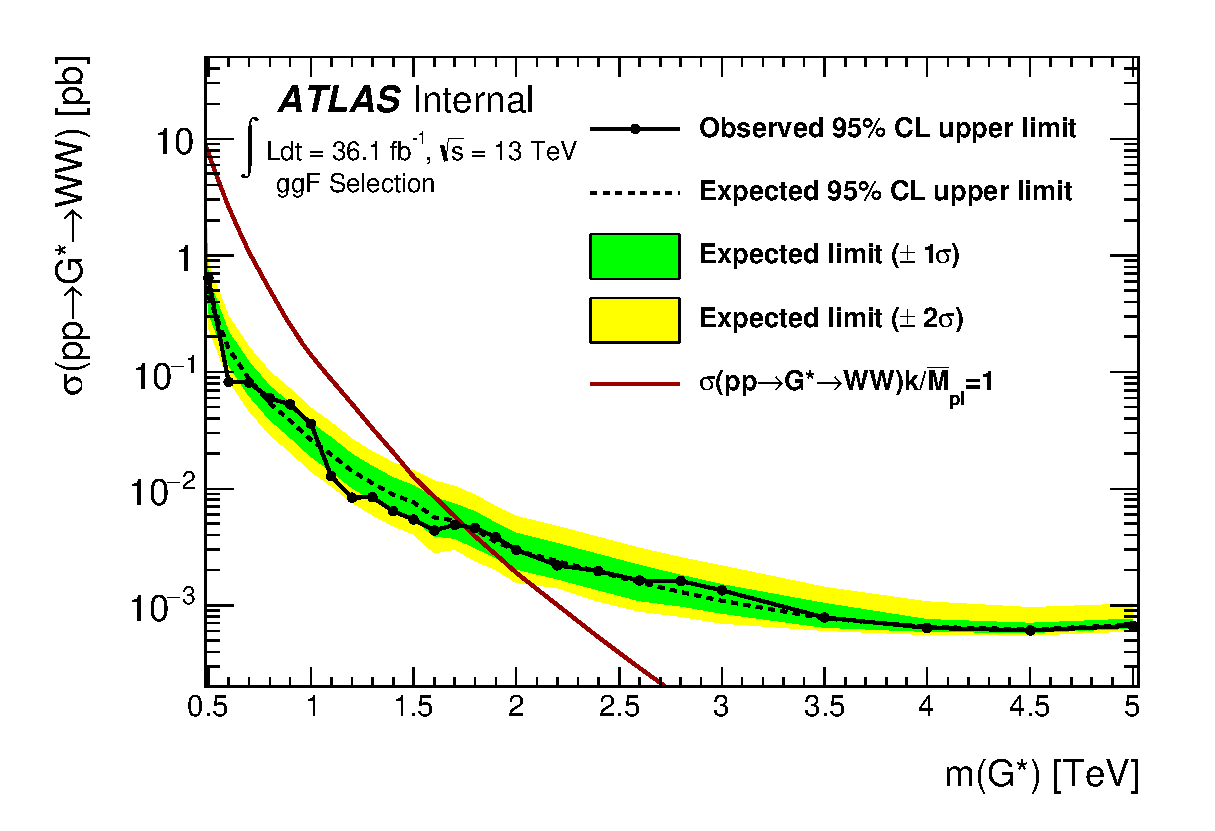
\includegraphics[width=0.8\textwidth]{figures/Results/new/final_lim/RSGWW_LPHP_ggF}\label{fig:lim_RSGWW:a}}\\
\subfloat[]{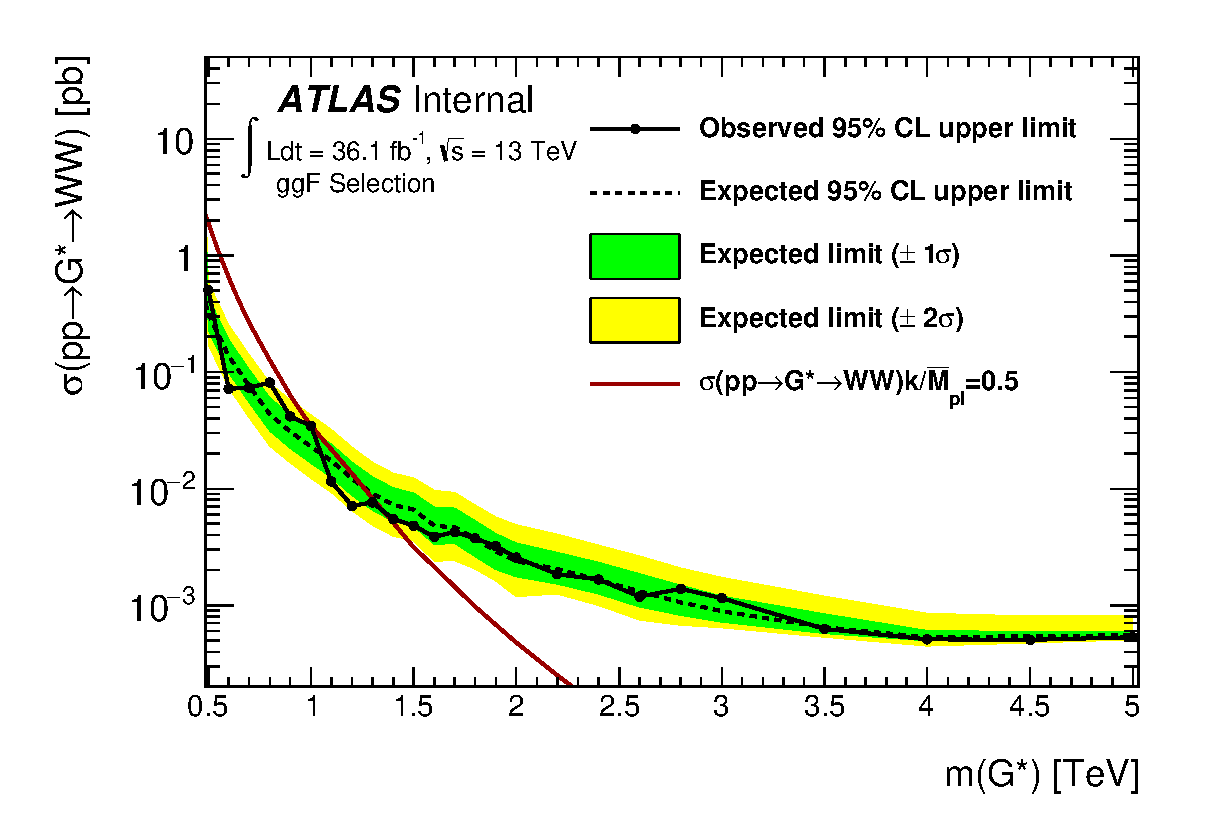
\includegraphics[width=0.8\textwidth]{figures/Results/new/final_lim/RSGWW_ReWeight_LPHP_ggF}\label{fig:lim_RSGWW:b}}\\
\caption[Observed and expected upper limits for RS $G^*$ model (gluon-gluon fusion selection)]{The observed and expected 95\,\% CL upper limits on cross section times branching ratio for RS $G* \rightarrow WW$ in the combined LP and HP signal regions, for the ggF selection, are shown for \protect\subref{fig:lim_RSGWW:a} $k/\overline{M}_{\rm Pl}=1.0$ and  \protect\subref{fig:lim_RSGWW:b} $k/\overline{M}_{\rm Pl}=0.5$. The theoretical cross sections for the signal models are overlaid. Limits are calculated with an asymptotic approximation for mass points below 1.6\,\TeV, and with pseudo-experiments above 1.6\,\TeV.}
\label{fig:lim_RSGWW}
\end{figure}
\begin{figure}[H]
\centering
\subfloat[]{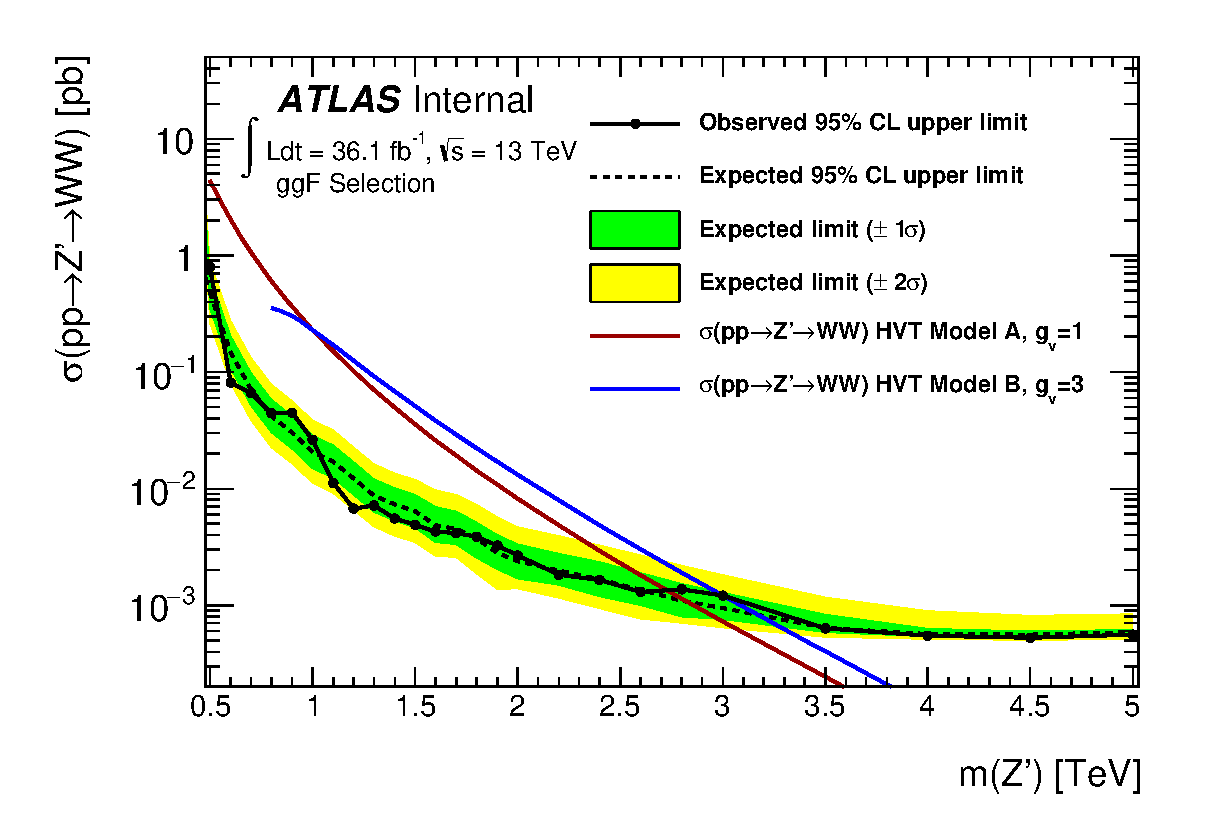
\includegraphics[width=0.8\textwidth]{figures/Results/new/final_lim/HVTWW_LPHP_ggF}\label{fig:lim_HVT:a}}\\
\subfloat[]{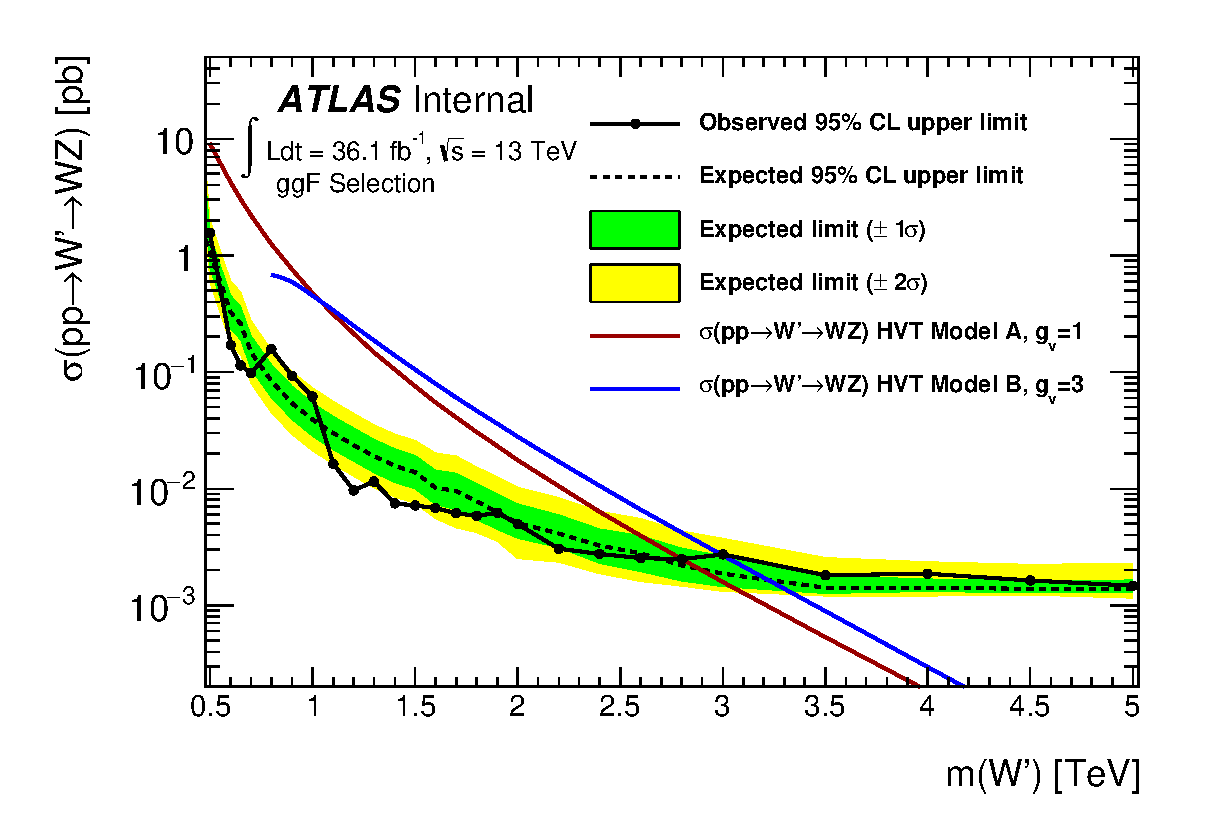
\includegraphics[width=0.8\textwidth]{figures/Results/new/final_lim/HVTWZ_LPHP_ggF}\label{fig:lim_HVT:b}}\\
\caption[Observed and expected upper limits for HVT $Z'$ and $W'$ model (gluon-gluon fusion selection)]{The observed and expected 95\,\% CL upper limits on cross section times branching ratio for \protect\subref{fig:lim_HVT:a} HVT $Z' \rightarrow WW$ and \protect\subref{fig:lim_HVT:b} HVT $W' \rightarrow WZ$, in the combined LP and HP signal regions, for the ggF selection. The theoretical cross sections for model-A ($g_V=1$) and model-B ($g_V=3$) are overlaid. Limits are calculated with an asymptotic approximation for mass points below 1.6\,\TeV, and with pseudo-experiments above 1.6\,\TeV.}
\label{fig:lim_HVT}
\end{figure}
\begin{figure}[H]
\centering
\subfloat[]{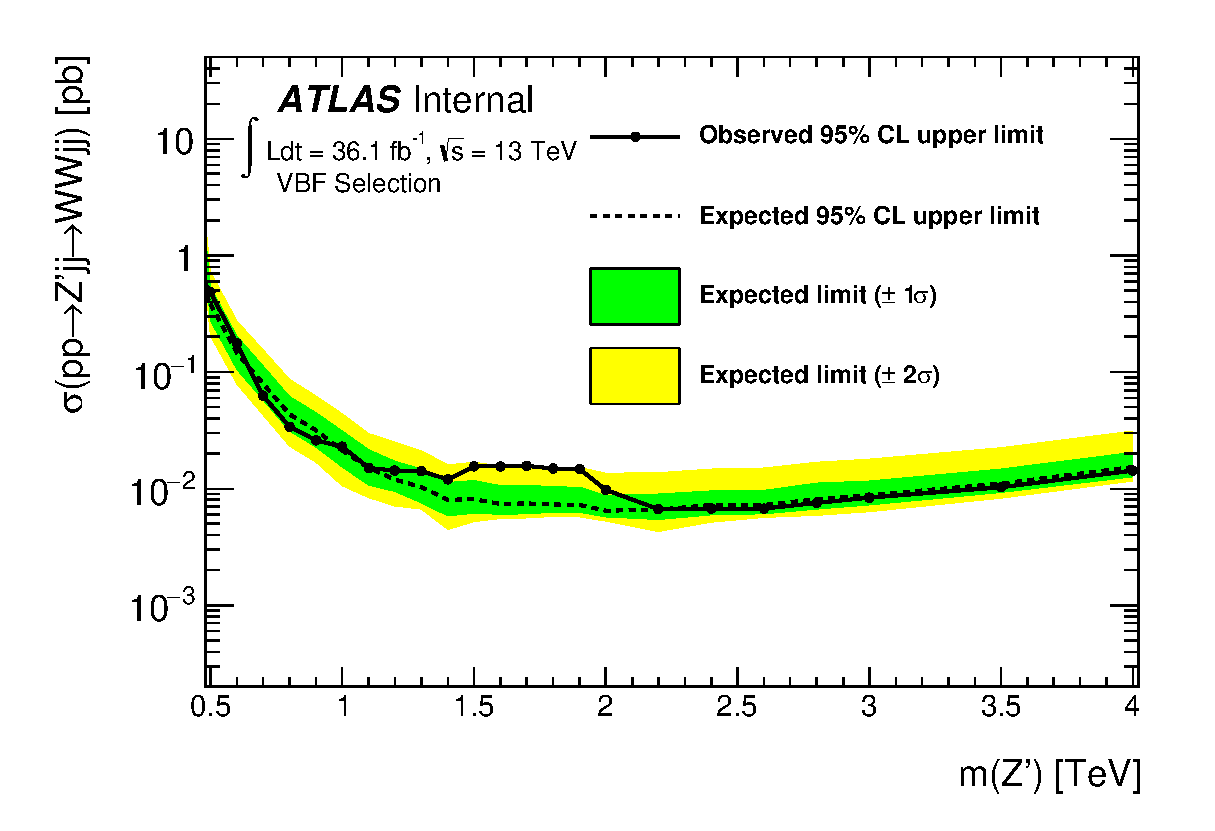
\includegraphics[width=0.8\textwidth]{figures/Results/new/final_lim/VBF_HVTWW_LPHP_VBF}\label{fig:lim_VBF_HVT:a}}\\
\subfloat[]{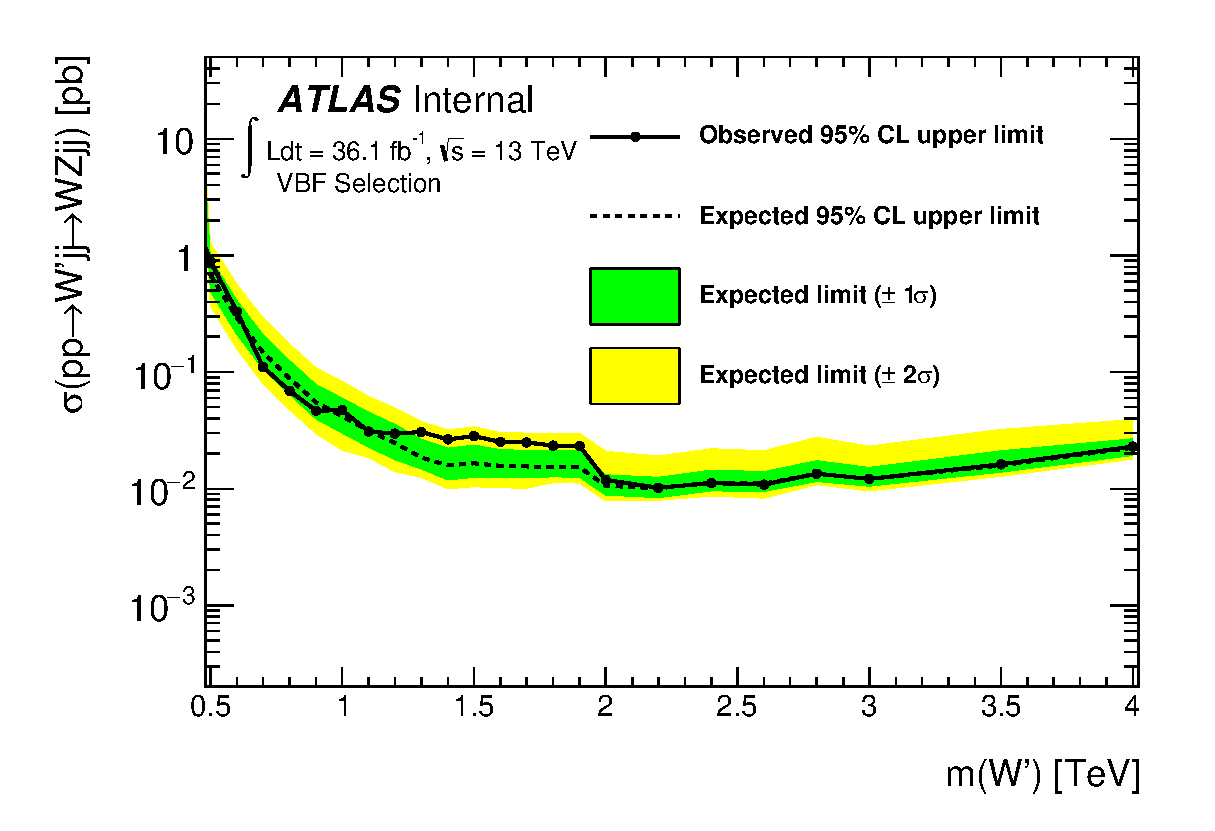
\includegraphics[width=0.8\textwidth]{figures/Results/new/final_lim/VBF_HVTWZ_LPHP_VBF}\label{fig:lim_VBF_HVT:b}}\\
\caption[Observed and expected upper limits for HVT $Z'$ and $W'$ model (vector boson fusion selection)]{The observed and expected 95\,\% CL upper limits on cross section times branching ratio for \protect\subref{fig:lim_VBF_HVT:a} HVT $Z' jj\rightarrow WWjj$ and \protect\subref{fig:lim_VBF_HVT:b} HVT $W'jj \rightarrow WZjj$, in the combined LP and HP signal regions, for the VBF selection. The mass region greater than 1.5\,\TeV\, is covered by two bins in the final discriminant, while the observed limit markers represent the tested signal points. Limits are calculated with an asymptotic approximation for mass points below 1.0\,\TeV, and with pseudo-experiments above 1.0\,\TeV.}
\label{fig:lim_VBF_HVT}
\end{figure}
\begin{figure}[H]
\centering
\subfloat[]{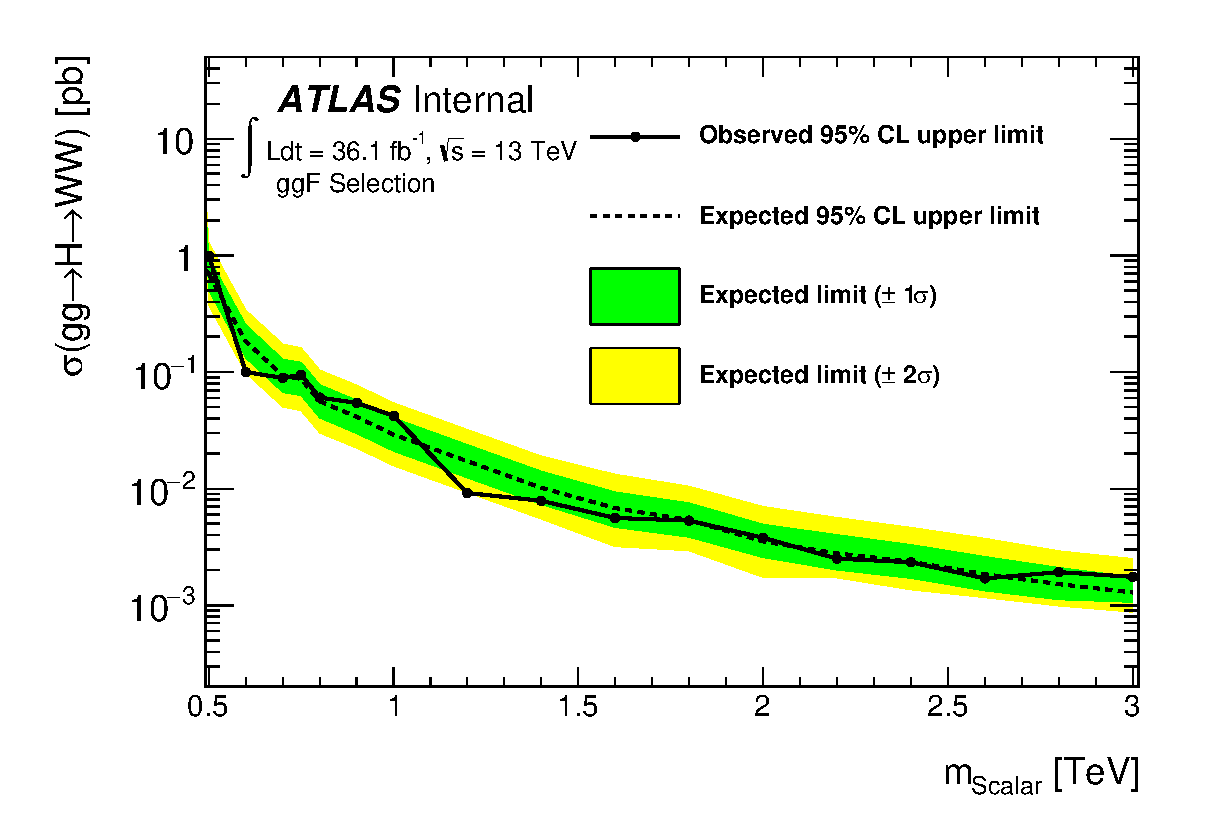
\includegraphics[width=0.8\textwidth]{figures/Results/new/final_lim/ggHWWNWA_LPHP_ggF}\label{fig:lim_scalar:a}}\\
\subfloat[]{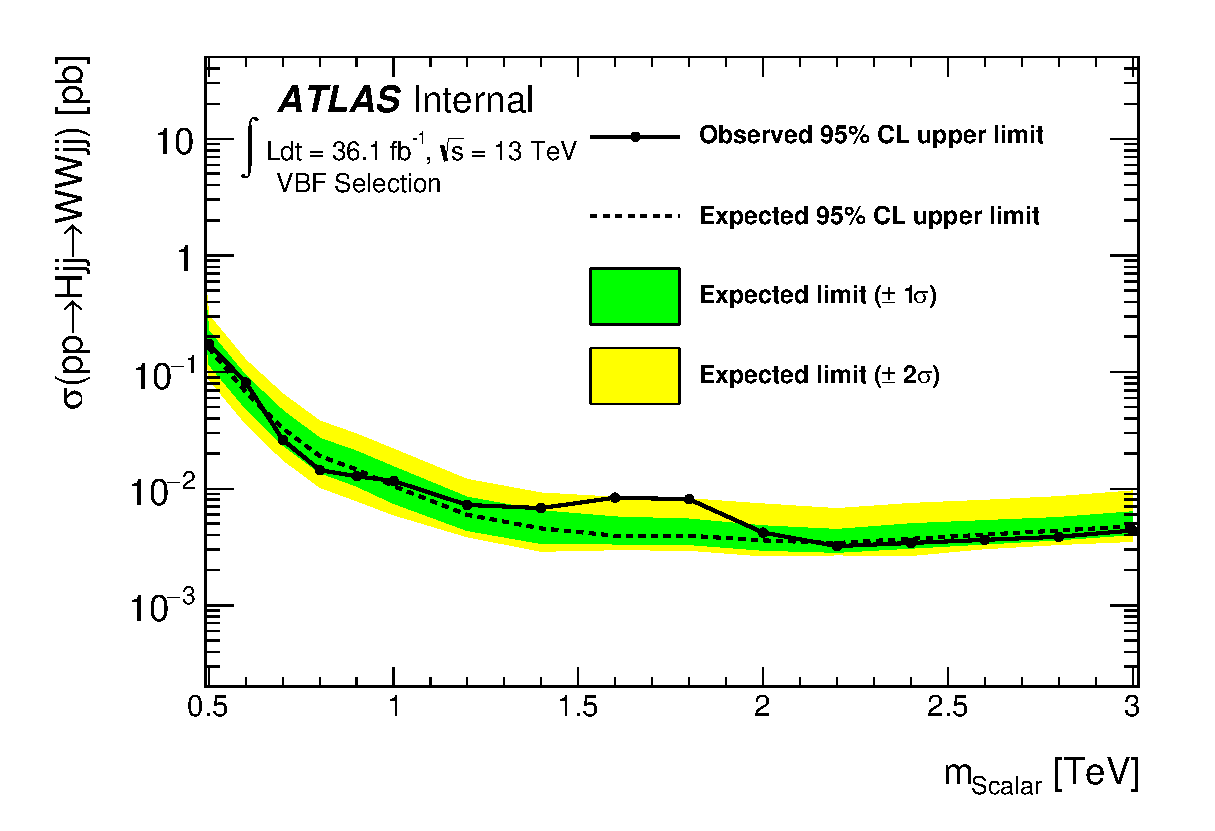
\includegraphics[width=0.8\textwidth]{figures/Results/new/final_lim/VBFWWNWA_LPHP_VBF}\label{fig:lim_scalar:b}}\\
\caption[Observed and expected upper limits for narrow, heavy Higgs model (gluon-gluon fusion and vector boson fusion selection)]{The observed and expected 95\,\% CL upper limits on cross section times branching ratio for a neutral heavy scalar (NWA) in the combined LP and HP signal regions, for the \protect\subref{fig:lim_scalar:a} ggF selection and \protect\subref{fig:lim_VBF_HVT:b} VBF selection. Signal samples generated with ggF (VBF) production are used for the ggF selection (VBF selection). The mass region greater than 1.5\,\TeV\, is covered by two bins in the final discriminant, while the observed limit markers represent the tested signal points. For the ggF (VBF) selection, limits are calculated with an asymptotic approximation for mass points below $1.6\,\TeV$\, ($1.0\,\TeV$), and with pseudo-experiments above $1.6\,\TeV$\,($1.0\,\TeV$).}
\label{fig:lim_scalar}
\end{figure}

The largest discrepancy between the expected and observed upper limits occur for signal models with VBF production, for masses between approximately $1.5-2.0\,\TeV$. The local $p$-values for the background-only hypothesis are shown in~\Fig{\ref{fig:p0}},  for the tested HVT $W'$ and $Z'$ signal models with VBF production. For the $Z'$ model, the maximum local significance, which does not take into account the look-elsewhere effect, is approximately $2.6\sigma$ for the fit at $m(W')=1.7\,\TeV$. In the post-fit plot for the HP SR with VBF selection (\Fig{\ref{fig:pf_hp_vbf}}), there are three events observed in the bin at 1.7\,\TeV, with less than one expected in the $WW$ channel. In the $WZ$ channel (which has a large overlap), three events are observed in the bin at 1.7\,\TeV\, as well, but the background expectation is slightly higher at $\sim1.5$ events. With only two bins covering the region $m(\ell\nu J)>1.5\,\TeV$, the larger than expected upper limits for tested mass points in this region are mostly due to the entries in this single bin.


\begin{figure}[H]
\centering
\subfloat[]{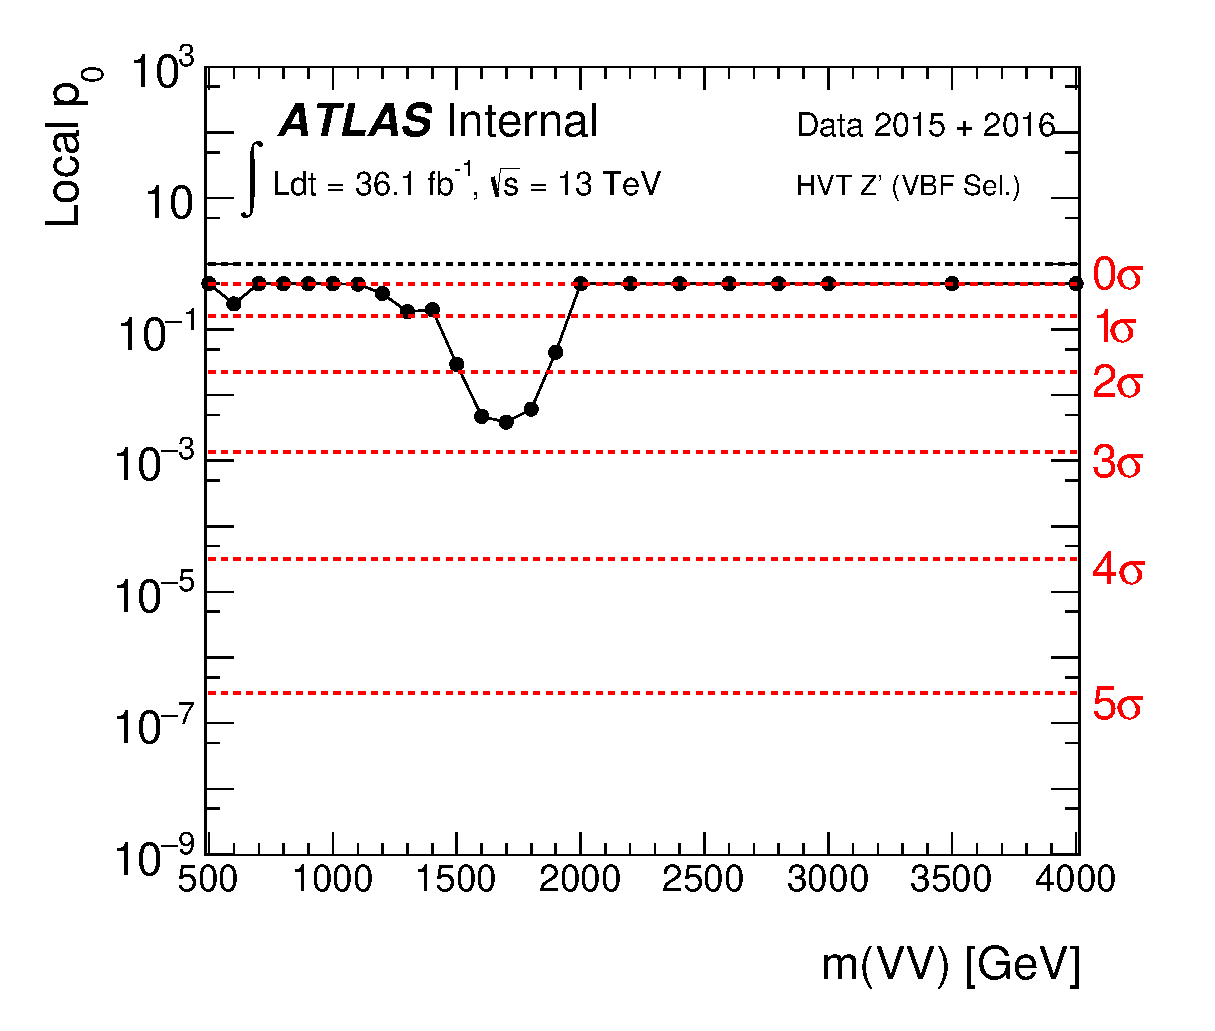
\includegraphics[width=0.49\textwidth]{figures/Results/new/final_lim/VVM_p0_VBF_HVTWW_VBF}\label{fig:p0:a}}
\subfloat[]{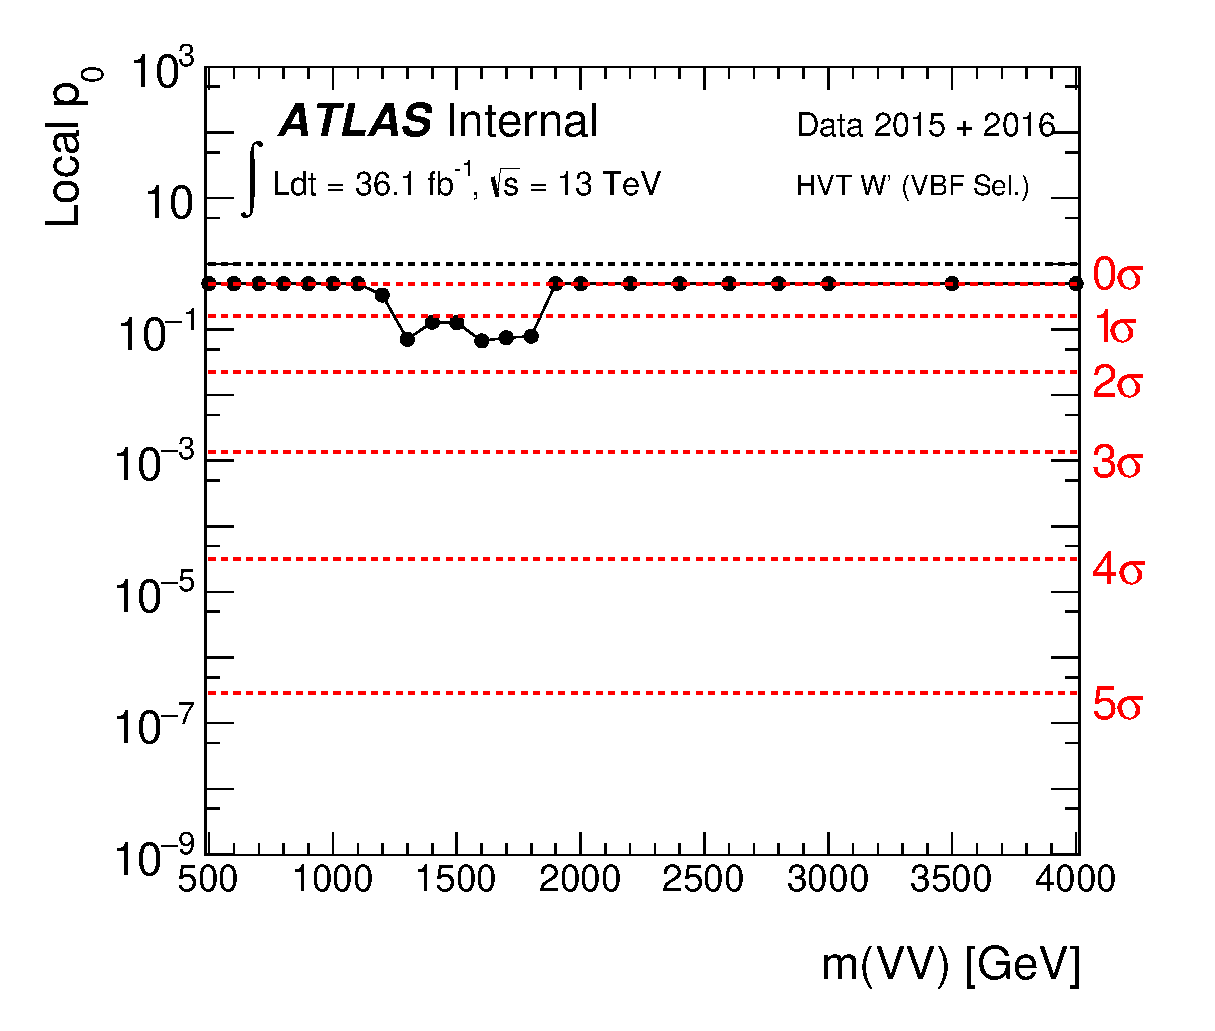
\includegraphics[width=0.49\textwidth]{figures/Results/new/final_lim/VVM_p0_VBF_HVTWZ_VBF}\label{fig:p0:b}}
\caption[Local $p$-value for HVT signal (vector boson fusion selection)]{Local $p$-value for the tested \protect\subref{fig:p0:a} HVT $W'$ and \protect\subref{fig:p0:b} HVT $Z'$ signal models. The mass region greater than 1.5\,\TeV\, is covered by two bins in the final discriminant. }
\label{fig:p0}
\end{figure}

%Excluded Masses
%\afterpage{\clearpage}
\section{Comparison with Previous Results}

Signal masses for which the theoretical cross section is larger than the observed cross section can be excluded at 95\,\% CL. The expected and observed excluded masses are shown in~\Tab{\ref{tab:excluded}}. The most recent CMS result~\cite{CMS_diboson_run2} included up to $2.7\,\ifb$\,of $pp$ data with center-of-mass energy $\sqrt{s}=13\,\TeV$, and excluded $W'$ and $Z'$ resonance masses below $2.3\,\TeV$\,($2.4\,\TeV$) for HVT model-A (model-B). The most recent ATLAS result~\cite{diboson_comb_2016} included $3.2\,\ifb$\, of $pp$ data with center-of-mass energy $\sqrt{s}=13\,\TeV$, and excluded $W'$ and $Z'$ resonance masses below $2.35\,\TeV$\,($2.6\,\TeV$) for HVT model-A (model-B). This thesis extends the excluded mass range from the ATLAS result by $450\,\GeV$\,($390\,\GeV$) for $W'$ resonances and by $380\,\GeV$\,($400\,\GeV$) for $Z'$ resonances in model-A (model-B).

The most recent ATLAS result excluded bulk RS graviton masses below $1.1\,\TeV$ for $k/\overline{M}_{\rm Pl}=1.0$, while this thesis extends the excluded mass range by $650\,\GeV$. Upper limits on production cross section times branching ratio to $VV=WW/ZZ$\footnote{
	 For heavy scalar models (NWA) and bulk RS $G^{*}$ models, the most recent results present upper limits on the cross section times branching ratio to $VV=WW/ZZ$. For comparison, the ratio of the $WW:ZZ$ decay is approximately $2:1$. Thus, upper limits for the $VV$ combined channel are approximately 1.5 times the upper limits for $WW$ channel presented here. 
} for a bulk RS $G^{*}$ with $k/\overline{M}_{\rm Pl}=0.5$ were set by CMS ranging from $1.2\,$pb ($600\,\GeV$) to $3\,$fb ($4\,\TeV$). This thesis improves upon those results and sets upper limits on cross section times branching ratio to $WW$ ranging from $0.5\,$pb (500\,\GeV) to $0.6\,$fb (5\,\TeV), and presents the first excluded mass range for a bulk RS graviton with $k/\overline{M}_{\rm Pl}=0.5$. 

ATLAS set upper limits on production cross section times branching ratio to $VV=WW/ZZ$ for a narrow scalar resonance ranging from $1\,$pb at $500\,\GeV$\,to $6\,$fb at $3\,\TeV$~\cite{diboson_comb_2016}. This thesis improves upon those results and sets upper limits on production cross section times branching ratio to $WW$ for a narrow scalar resonance ranging from $0.2\,$pb at $500\,\GeV$\,(model with VBF production) to $1.8\,$fb at $3\,\TeV$\,(model with ggF production). Finally, the first upper limits on production cross section times branching ratio to $WV$ are set for HVT $W'$ and $Z'$ resonances with VBF production.
%
% Excluded Masses
\begin{table}[htb]
\centering
\begin{tabular}{l|c|c}
\hline\hline
\textbf{Signal Model}\quad\quad\quad\quad\,&\multicolumn{2}{c}{\textbf{Excluded Masses at 95\,\% CL}}\\\hline%\cline{2-3}
$WZ$ Selection&Expected [\GeV]&Observed [\GeV]\\\hline
%&&\\
\rule{0pt}{2.5ex}\,\,\,HVT $W'$&&\\
\,\hfill Model A ($g_v=1$)&$<2880$&$<2800$\\
\,\hfill Model B ($g_v=3$)&$<3220$&$<2990$\\\hline
\multicolumn{3}{c}{\,}\\\hline
$WW$ Selection\quad\quad\quad\quad\,&Expected [\GeV]&Observed [\GeV]\\\hline
\rule{0pt}{2.5ex}\,\,\,HVT $Z'$&&\\
\,\hfill Model A ($g_v=1$)&$<2830$&$<2730$\\
\,\hfill Model B ($g_v=3$)&$<3170$&$<3000$\\
\rule{0pt}{2.5ex}\,\,\,RS $G^*$&&\\
\,\hfill $k/\overline{M}_{\rm Pl}=1.0$&$<1740$&$<1750$\\
\,\hfill $k/\overline{M}_{\rm Pl}=0.5$&$<1250$&$<980$ and $1020-1350$\\
\hline\hline
\end{tabular}
\caption[Observed and expected excluded masses at 95\,\% confidence level]{Observed and expected excluded masses at 95\,\% CL for HVT $W'$, HVT $Z'$, and RS $G^*$ signal models.}
\label{tab:excluded}
\end{table}


\clearpage


